%!TEX root = ../lectures_olympics.tex


\chapter{几何光学}

 \begin{wrapfigure}{o}{6cm}
 	\includegraphics[width=6cm]{images/opt-20.pdf} 
 	\caption{Hubble 空间望远镜}\label{fig: }
 \end{wrapfigure}
经过一百多年的努力,从牛顿开始人们逐步认识到了光的本质。
光是传递电磁相互作用的物理对象,在实践上它具有多面性,有时它像一个个不可分割的颗粒一样与其它粒子碰撞或被发射和吸收,有时又像波一样向全空间发散,这就是我们所谓的波粒二象性。
光学现象具有复杂的一面,在研究过程中人们往往首先关注光在特定物理过程中的主要性质,随着深入再来考虑光的其它性质。
在一些过程当中,光的粒子性质表现得比波动性质要多一些,这时光可以看成是许多以光速运动的微观粒子---{\heiti 光子}(photon)在空间当中运动,这时光子运动的轨迹就是我们通常所谓的{\heiti 光线}(light ray)。

对光线的研究就构成了几何光学的主要内容,在几何光学中首先忽略光的波动性质而关注光的运动轨迹。这可以看成是光的波长远小于光学仪器尺寸时的极限。
对光线的研究可以使我们认识到光的部分性质,并利用这些性质来制造光学仪器来帮助我们的眼睛,使我们能够看到那些肉眼无法看到的对象,极大地扩充了人类对微观世界和宇宙的认识。

经验告诉我们在均匀介质当中光沿着直线传播,当介质不均匀或光射到两种不同介质的分界面上时,光线会偏离直线进行传播。
根据偏转性质的不同,将这些现象称为{\heiti 反射}(reflection)、{\heiti 折射}(refraction)、{\heiti 散射}(diffraction)、{\heiti 吸收}(absorption)等光学现象。
下面就来看一些典型的光学现象。


\section{光的反射}
当光射在平整的表面上时有可能发生反射。
光在平面镜上的{\heiti 反射定律}(Law of Reflection)比较简单,如图所示光射在平面镜上的$P$点,过$P$点做平面镜的垂线$PQ$称为入射光的法线,线$AP$为入射光,入射光与法线的夹角$\alpha$为入射角,反射光$PB$与法线的夹角$\beta$称为反射角,反射定律指出反射光和入射光在一个平面上,入射角等于反射角$\alpha=\beta$。



\begin{figure}
\begin{center}
\includegraphics[width=0.4\textwidth]{images/reflection.pdf}
\end{center}
\end{figure}

\begin{example}
如图所示,$AB$表示一平直的平面镜,$P_1P_2$是水平放置的米尺(有刻度的一面朝着平面镜),$MN$是屏,三者相互平行,屏$ MN$上的$ ab$表示一条竖直的缝(即$ ab$之间是透光的)。
某人眼睛紧贴米尺上的小孔$ S($其位置如图所示),可通过平面镜看到米尺的一部分刻度。试在本题图上用三角板作图求出可看到的部
位,并在$P_1P_2$上把这部分涂以标志。
	\begin{center}
		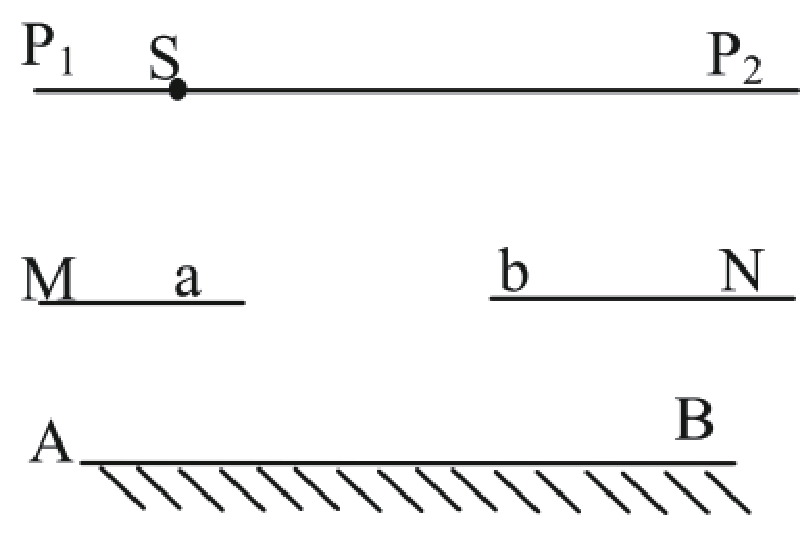
\includegraphics[width = 0.4\textwidth]{images/opt-1.pdf} 
	\end{center}
\tagged{student}{\vspace*{0cm}}
\begin{taggedblock}{teacher}
\noindent
解析:略
\end{taggedblock}
\end{example}


\begin{example}
两个平面镜之间的夹角为$45^\circ$,$60^\circ$,$120^\circ$。而物体总是放在平面镜的角等分线上。试分别求出像的个数。
	\begin{center}
		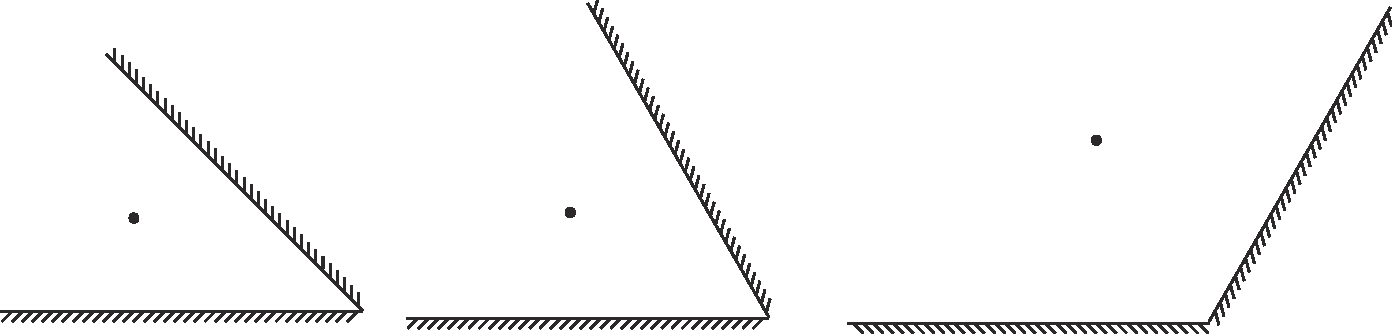
\includegraphics[width = 0.9\textwidth]{images/opt-2.pdf} 
	\end{center}
	\begin{taggedblock}{teacher}
		\noindent
		解析:7,5,2
	\end{taggedblock}
\end{example}

%%%%%%%%%%%%%
\begin{example}
	两镜面间夹角$\alpha =15^\circ$,$OA=10\si{cm}$,$A$点发出的垂直于$L_2$ 的光线射向$L_1$后在两镜间反复反射,直到光线平行于某一镜面射出,则从$A$点开始到最后一次反射点,光线所走的路程是多少。
		\begin{center}
			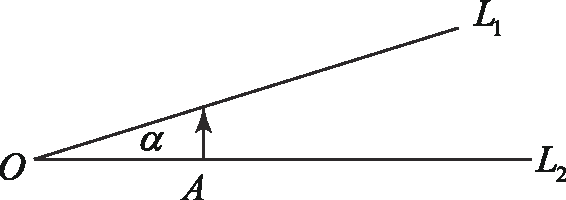
\includegraphics[width = 0.4\textwidth]{images/opt-3.pdf} 
		\end{center}
	\tagged{student}{\vspace*{4cm}}
	\begin{taggedblock}{teacher}
		\noindent
		解析:$\frac{10}{\cos75\si{\degree}}$
	\end{taggedblock}
\end{example}
%%%%%%%%%%%%%%%%%%%%

当光在弯曲表面上光的反射定律与平面镜相同,但是需要在光的入射点上做出反射面的切平面,通过入射点做垂直于切平面的直线就是入射光的法线。
反射光线位于由入射光和法线所决定的平面内,并且反射角等于入射角。





\begin{example}
如图所示有一个球面反射镜,其半径为$R$,中心位于$O$点处。
一束平行于对称轴$M$、与其相距$d$的入射光线被球面镜反射以后与$MN$相交于$B$点,求$OB$的距离$x$。
\begin{flushright}
\includegraphics[width=0.4\textwidth]{images/sphirical-mirrow-reflaction.pdf}
\end{flushright}
\tagged{student}{\vspace*{2cm}}
\begin{taggedblock}{teacher}
\noindent
解析:连接$O$点和光的入射点$S$,这就是该光线反射的法线,记角$ASO$为$\alpha$,根据反射定律反射角$OSB$也是$\alpha$。
过$O$做$AS$的第一线$OD$,在三角形$OSD$当中根据定义可得
\[
\sin\alpha=\frac{d}{R}
\]
在三角形OSB当中用正弦定理
\[
\frac{x}{\sin\alpha}=\frac{R}{\sin 2\alpha}
\]
将上式化简可得
\[
x=\frac{\sin\alpha}{\sin 2\alpha}R=\frac{1}{\sqrt{1-\left (\frac{d}{R}\right )^2}}\frac{R}{2}
\]
从中可以看出反射光与交轴的交点与$d$有关。
但是如果$d\ll R$的话依然可以近似认为所有光线都会聚到$\frac{R}{2}$处。
以此可以引出近轴光线成像。
\end{taggedblock}
\end{example}


\section{折射与全反射}
当光射向透明的介质时,情况要稍复杂一些。
这时一部分光线按照反射定律被反射以外,还会有一部分光线进入到介质当中,当光射入介质时它的传播方向有可能发生变化,也就是光线会偏折。
将光进入介质并且发生偏转的现象称为光的{\heiti 折射}\footnote{光可以看做是某种形式能量的传播,除了反射和折射以外还可以被物质吸收一部分}。
\subsection{折射定律(Law of Refraction)}
\begin{figure}[hbtp]
\begin{center}
\includegraphics[width=0.5\textwidth]{images/refraction.pdf}
\label{fig: geo-refraction}
\caption{光的折射,入射角和折射角正弦之比等于常数}
\end{center}
\end{figure}

如图\ref{fig: geo-refraction} 所示的光线在两种均匀介质的分界面上发生偏转,折射定律告诉我们,入射角$\alpha$与折射角$\beta$的正弦之比为常数$n_{12}$
\begin{equation}\label{eqn: geo-refraction law}
\frac{\sin\alpha}{\sin\beta}=n_{12}
\end{equation}
该常数称为两个介质之间的相对折射率,下标代表特定的两种介质。
如果两种介质之一为真空,此时折射定律当中的$n$称为另外一种介质的{\heiti 绝对折射率},或{\heiti 折射率}(index, indices)。

折射率与光在给定介质当中的速度有关,在真空当中光速永远不变,记作$c$。
当光在某种介质当中的速度为$v<c$时,可以证明该介质的绝对折射率
\begin{equation}
n=\frac{c}{v}>1,
\end{equation}
光在绝对折射率为$n_1$和$n_2$的两种透明介质之间的相对折射率$n_{12}$可以由它们各自的绝对折射率所导出:
\begin{equation}
n_{12} = \frac{n_2}{n_1},
\end{equation}
这样光在两个介质之间的折射定律也可写成更对称的形式
\begin{equation}
n_1\sin\alpha = n_2\sin\beta,
\end{equation}
在实际使用过程当中上式更为方便。

\begin{example}
一个大游泳池,池底是水平面,池水深$ 1.2\si{m}$,有一直杆竖直立于池底,浸入水中部分杆是杆全长的一半,当太阳光以与水平方向成$ 37^\circ$角射在水面上时,测得杆在池底的影长为$ 2.5\si{m}$,求水的折射率。
\tagged{student}{\vspace*{3cm}}
\begin{taggedblock}{teacher}
\newline
解析:$\frac{4}{3}$
\end{taggedblock}
\end{example}


和反射的情况类似,当在弯曲的介质表面折射时,也是需要首先找到入射点上两种介质分界表面处的切平面,进而找到法线,再通过折射定律来判断折射光线的方向或其它相关物理量。
\begin{example}
用折射率为$ n $的透明物质做成内、外半径分别为$ a$、$b $的空心球,如图所示,球的内表面涂有能完全吸收光的物质,则当一平行光射向此球时,球吸收的光束的横截面积多大(指光束进入空心球前的横截面积)?
	\begin{flushright}
		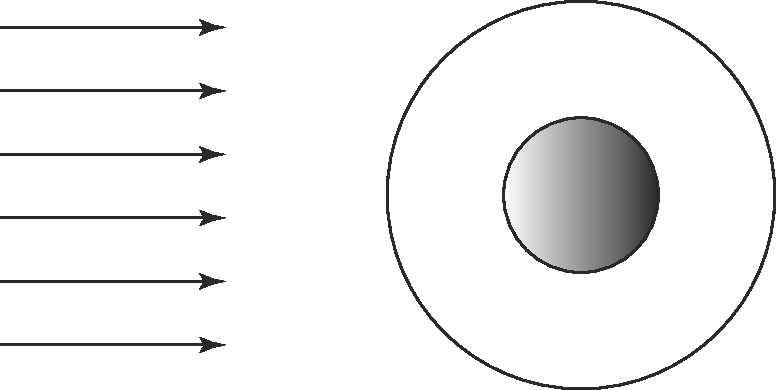
\includegraphics[width = 0.4\textwidth]{images/opt-4.pdf} 
	\end{flushright}
\tagged{student}{\vspace*{4cm}}
\begin{taggedblock}{teacher}
\noindent
解析:若$na<b$:$S=\pi n^2a^2$,否则$S=\pi b^2$
\end{taggedblock}
\end{example}

%%%%%%%%%%%%%
\begin{example}
	内表面只反射而不吸收光的圆筒内有一半径为$ R $的黑球,距球心为$ 2R $处有一 点光源$ S$,球心$O$和光源$ S$皆在圆筒轴线上,如图所示。
	若使点光源向右半边发出的光最后全被黑球吸收,则筒的内半径$ r $最大为多少?
	\tagged{student}{\vspace*{2cm}}
		\begin{flushright}
			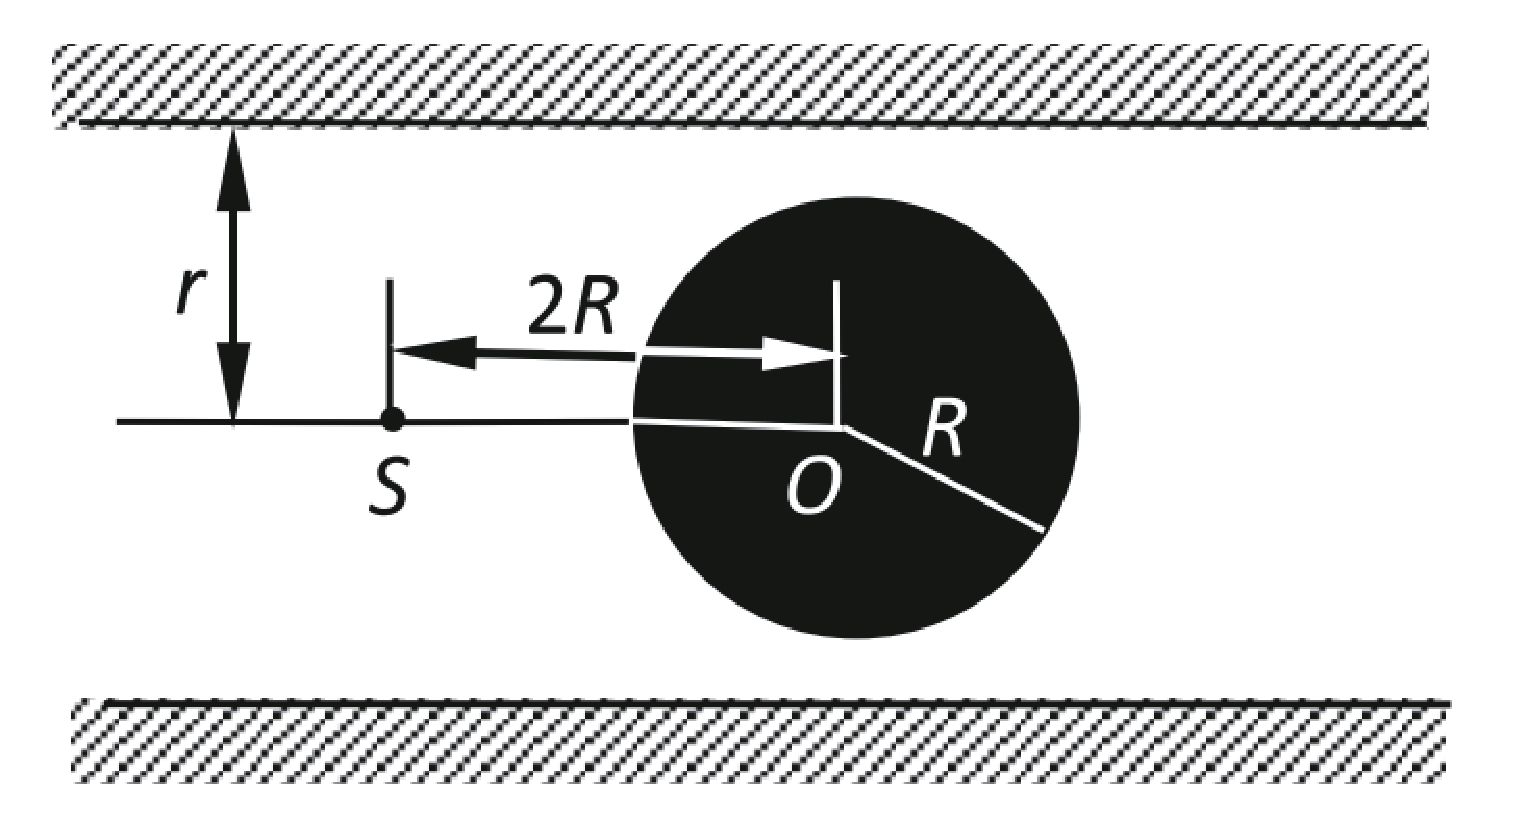
\includegraphics[width = 0.3\textwidth]{images/opt-15.pdf} 
		\end{flushright}
	\begin{taggedblock}{teacher}
		\noindent
		解析:$\frac{2R}{\sqrt{3}}$
		\begin{figure}[hbtp]
					\includegraphics[width = 0.5\textwidth]{images/opt-4-5.pdf}
				\end{figure}
	\end{taggedblock}
\end{example}
%%%%%%%%%%%%%%%%%%%%

\subsection{全反射}
我们知道光路是可逆的,折射现象当中也不例外。
考虑如图\ref{fig: geo-refraction}所示的折射,对于两种介质之间的任何一条折射光线在介质1当中的角度$\alpha$都大于在2中的角度$\beta$,两者之间有一个明显的不对称性。
习惯上称介质1为光疏介质,介质2为光密介质,从定义可以看出当光在两种不同折射率的介质之间的折射时,其中折射率较小的介质为光疏介质,折射率较大的介质则是光密介质。
$\alpha$角最大的可能取值为$90^\circ$,此时应对着的介质2中的角度$\beta_0$为
\begin{equation}
\beta_0 = \arcsin\left (\frac{1}{n}\right )
\end{equation}
根据光路的可逆性,介质2当中以$\beta_0$入射光线的折射角就是$90^\circ$,对于任何大于$\beta_0$的入射角通过折射定律\ref{eqn: geo-refraction law}计算出的折射角没有意义。
实际发生的情况则是所有大于$\beta_0$的入射光线都被反射回来,而没有折射光\footnote{波动光学告诉我们,准确的说,折射光是一种{\heiti 倏逝波}(evanescent wave),它随着透射深度指数衰减,并且在介质分界面下几个波长处几乎消失}。
这种现象称作光的全内反射或{\heiti 全反射}(total internal reflection),能够发生全反射最小的入射角$\beta_0$称作两个介质之间全反射的{\heiti 临界角}(critical angle)。
很明显,只有光从光密介质向光疏介质入射时才有可能发生全反射现象。

\begin{example}
用临界角为$42^\circ$的玻璃制成的直角三棱镜ABC,$\beta=15^\circ$,一束光线垂直$AC$面射入,如图所示,求它在棱镜内发生全反射的次数。
	\begin{flushright}
		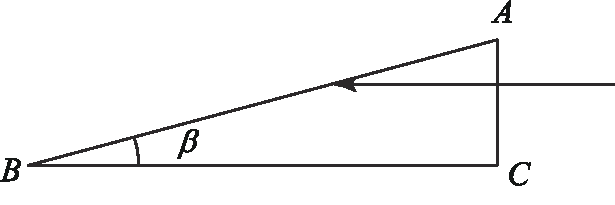
\includegraphics[width = 0.5\textwidth]{images/opt-6.pdf} 
	\end{flushright}

\tagged{student}{\vspace*{1cm}}
\begin{taggedblock}{teacher}
\noindent
解析:2
\end{taggedblock}
\end{example}




\begin{example}
图是光导纤维的示意图。$AB$为其端面,纤维内芯材料的折射率$n$,试问入射角在什么范围内才能确保光在光导纤维内传播?
	\begin{flushright}
		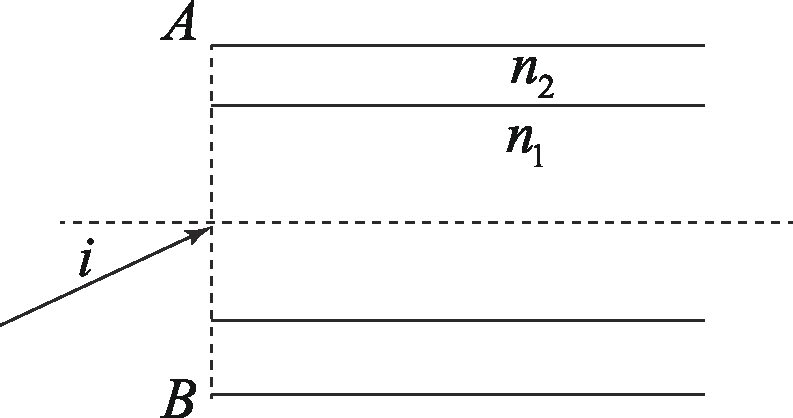
\includegraphics[width = 0.4\textwidth]{images/opt-5.pdf} 
	\end{flushright}
\tagged{student}{\vspace*{4cm}}
\begin{taggedblock}{teacher}
\noindent
解析:$\sin i\leq\sqrt{n_1^2-n_2^2}$
\end{taggedblock}
\end{example}


%%%%%%%%%%%%%
\begin{example}
横截面为矩形的玻璃棒被弯成如图所示的形状,一束平行光垂直地射入平表面$A$上。试确定通过表面$A$进入的光全部从表面$B$射出的$ R/d$的最小值。已知玻璃的折射为 1.5。
	\begin{flushright}
		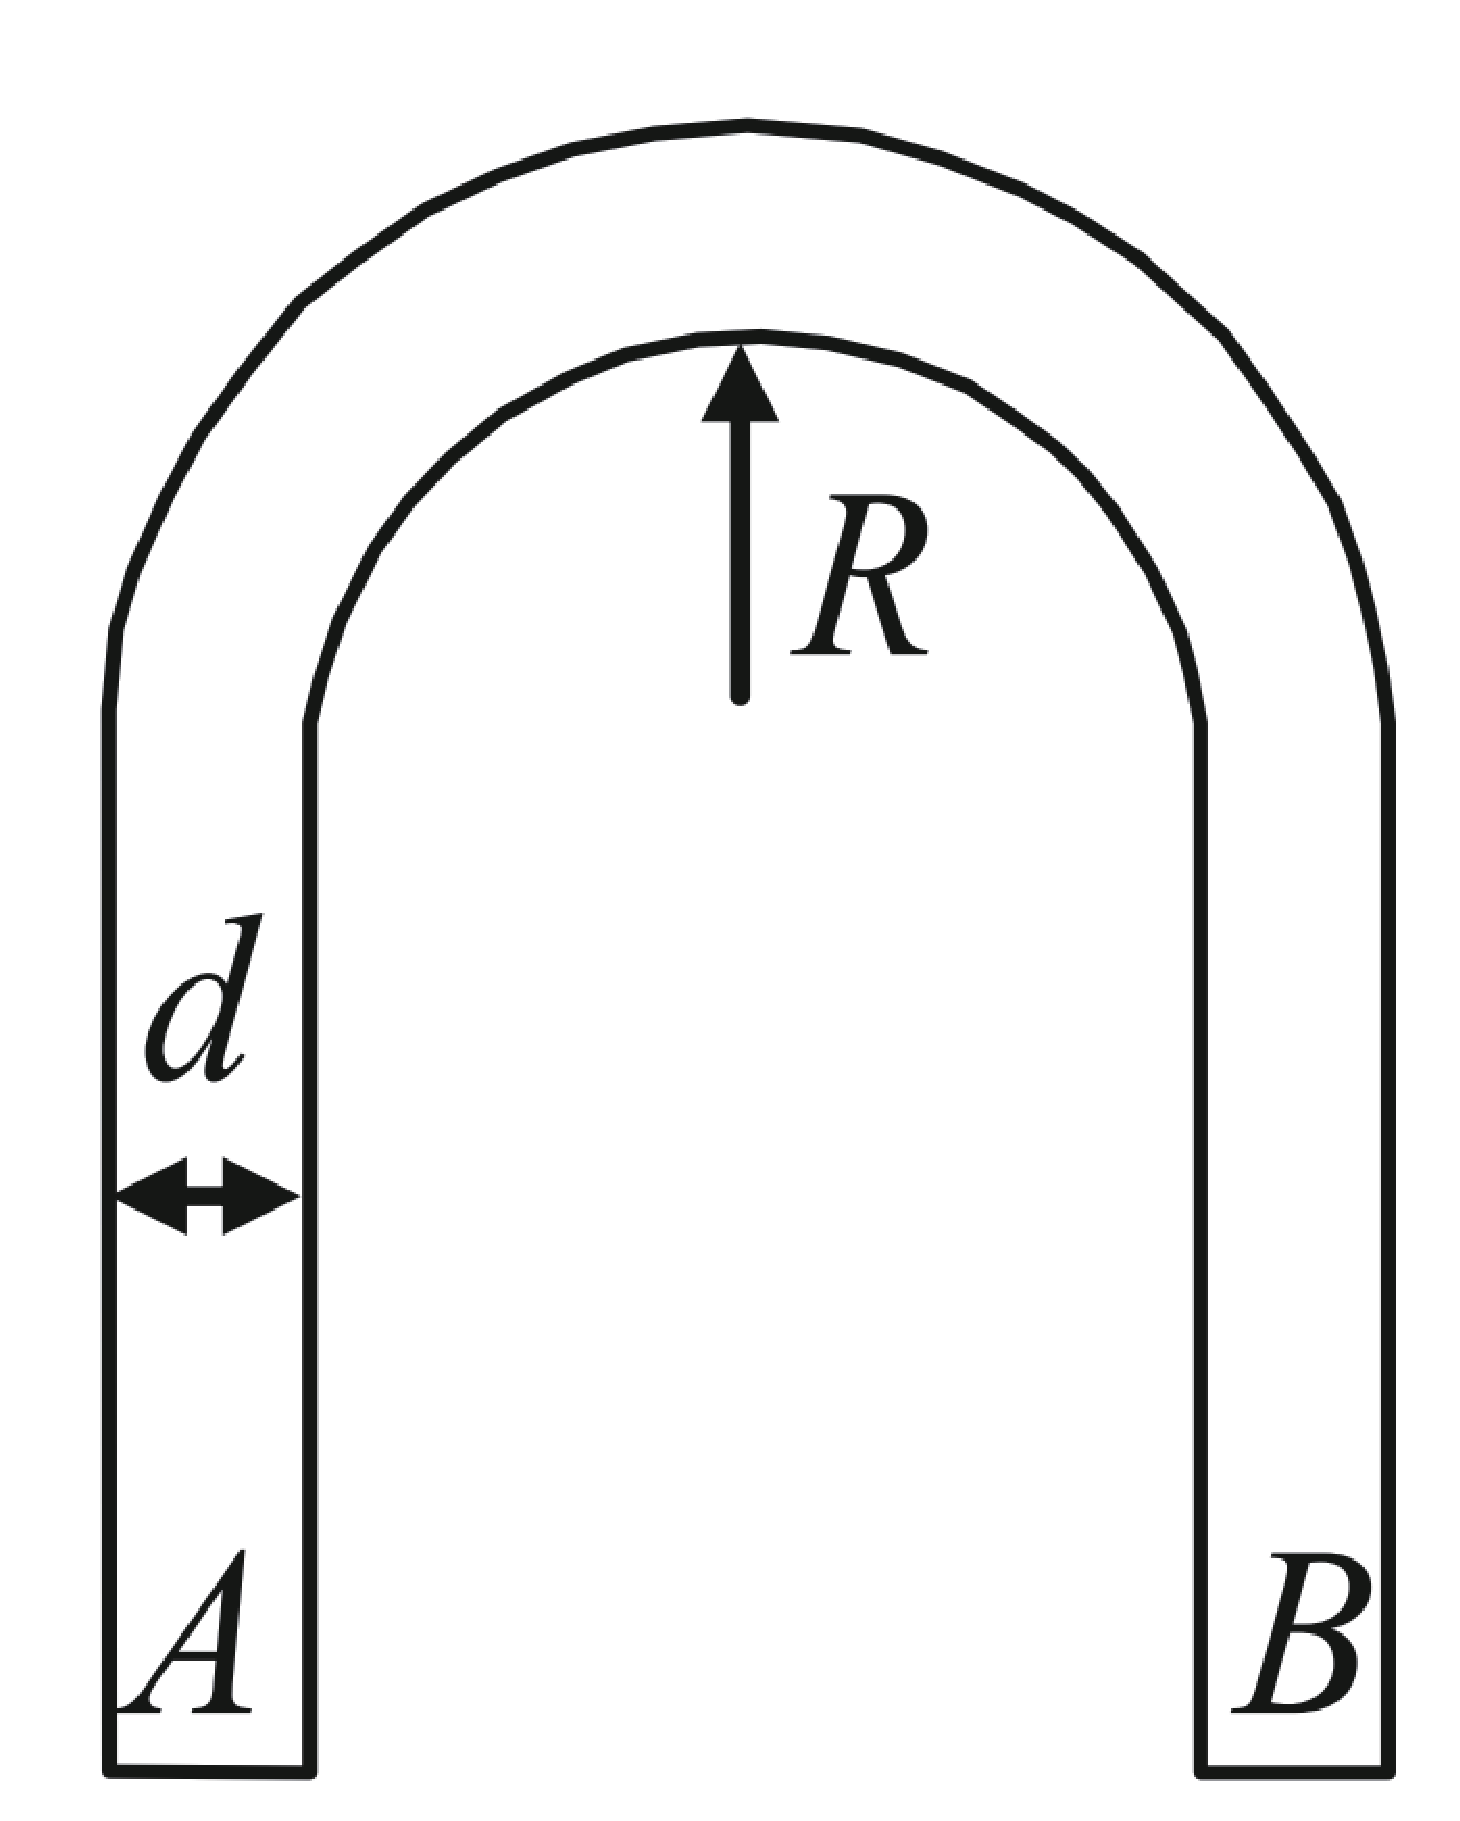
\includegraphics[width = 0.3\textwidth]{images/opt-7.pdf} 
	\end{flushright}
	\tagged{student}{\vspace*{0cm}}
	\begin{taggedblock}{teacher}
		\noindent
		解析:$\frac{1}{n-1}$
	\end{taggedblock}
\end{example}
%%%%%%%%%%%%%%%%%%%%





\section{光线传播的一般规律:惠更斯-菲涅尔原理和费马原理}

依靠光的反射和折射定律能够解释光在均匀介质以及两种均匀介质之间的传播,甚至从上面的例子当中还能看到能够解决一类不均匀介质当中的传播问题。
而在解决光在处处非均匀的介质当中的传播问题,例如真实空气当中的光的轨迹时显得更加复杂,
大气的折射率与空气密度有关,对于最一般的情况在不同地区、不同高度处的空气密度都有可能不同,我们很清楚、也很容易观察到光是以某种曲线在空气当中传播,这种情况下折射定律显得过于简单,如果不把折射定律推广到更加普遍的形式\footnote{这个推广得出了著名的{\heiti 光线方程}(Eikonal Equation)},是不可能求解光的传播轨迹的。

而著名的{\heiti 惠更斯-菲涅尔原理}(Huygens-Fresnel Principle)能够帮助我们更简单地回答和解决这类问题,它是一种基于光的波动性来决定光的传播方式的原理。
惠更斯认为,光是一种类似于水波的对象,当某一位置的水受到扰动以后,就会有水波向外扩散。
某一时候水波的形状称为水波的{\heiti 波阵面},对于光来说也一样,一个光源发出的光会在某一时候传播到一个曲面,就是光的波阵面。
波阵面的形状依赖于介质当中的波速,不难证明如果介质是均匀的,也就是说各点处的波速均相同,那么一个点状波源发出波的波阵面必然为同心圆;如果介质不均匀则波阵面会变成其它形状。
惠更斯原理指出,行进中的波阵面上任一点都可看作是新的次波源,而从波阵面上各点发出的许多次波所形成的包络面,就是原波面在一定时间内所传播到的新波面。
依据惠更斯原理能够在任意的介质中求解光线,只需要注意到从一个点光源发出的一条光线是各个波阵面的公垂线。


从惠更斯原理出发还能够得到光线传播满足的更外一条等价的原理:{\heiti 费马原理}(Fermat's Principle)。
费马原理指出:光在任意介质中从一点传播到另一点时,沿所需时间为极值\footnote{准确的说:当光路有一个十分小的变化量时,时间的一阶变化量为零}的路径传播。
可以认为费马原理是惠更斯原理在纯粹几何光学范围内的等价原理,它与惠更斯原理表达相同的物理含义,只不过一个用波的语言,另一个用光线的语言而已\footnote{由光的波动性出发可以通过惠更斯原理导出了几何光学的费马原理,在力学当中人们很早就注意到了另一个极值原理:最小作用量原理,它表明对于所有可能的运动,真实的运动是那条“动能减去势能对时间的积分”这样的量取极值。很长时间以来人们一直认为在它背后有一个波动性的解释,而这个解释最终被理论物理学家费曼所发现,物理上称为路径积分,感兴趣的同学可以去了解一下路径积分是如何进一步增加人们对微观世界运动规律的认识。}。
在折射率为$n$的均匀介质当中,光通过一段长度为$L$的距离所需要的时间为
\begin{equation}
t=\frac{L}{v}=\frac{L}{c/n} = \frac{1}{c}(nL),
\end{equation}
可以看出光传播所需要的时间正比于折射率与对应路程几何长度的乘积,习惯上将这个乘积称为{\heiti 光程}(path length),这样费马原理还可以表述为:光在任意介质中从一点传播到另一点所走光路的光程为极值,它可能是极大值,也可能是极小值,甚至是稳定值。


\begin{example}
利用费马原理解释光的反射和折射定律
	\begin{flushright}
		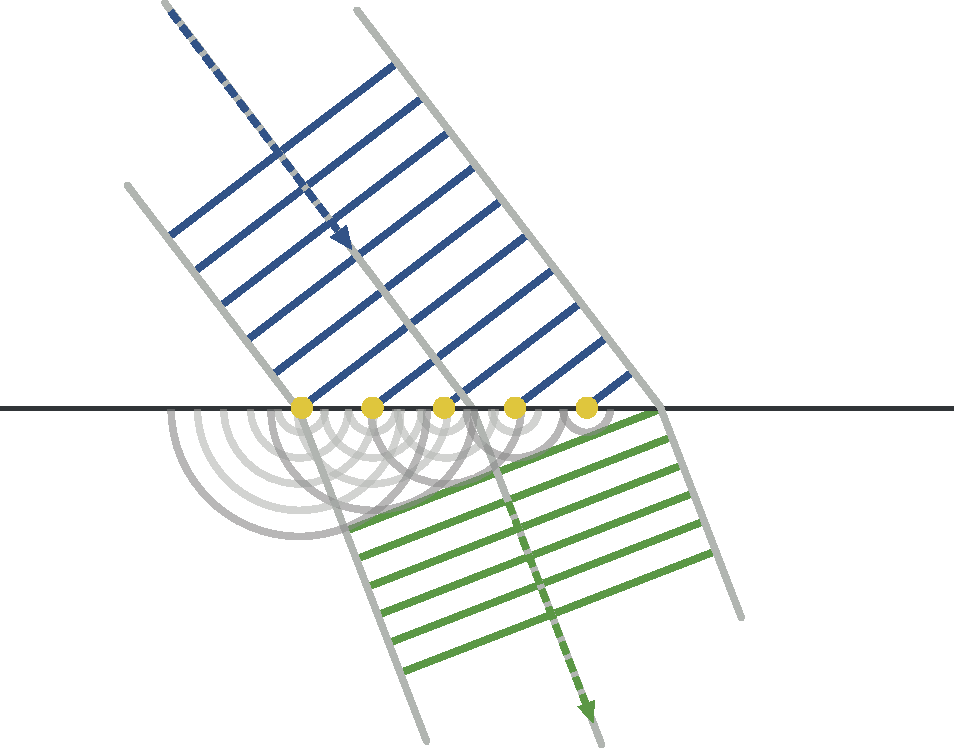
\includegraphics[width = 0.3\textwidth]{images/opt-19.pdf} 
	\end{flushright}
\tagged{student}{\vspace*{3cm}}
\begin{taggedblock}{teacher}
\noindent
\includegraphics[width=0.9\textwidth]{images/fermat-solution.pdf}

\noindent
解析:反射定律容易证明,但要注意的是要注意到从图中A点直接运动到B点的光线,它对应于另外一种可能的路线,费马原理实际上说的是真实传播的光线是同那些与它们非常接近的光线相比光程为极值的光线,并不是与所有可能的光线相比!
如左图所示,做B点的镜像点B',很容易证明从A经过P到达B的光程为最短,其它路线的光线的光程AP'+P'B'根据三角形的性质,两条边之和大于第三边,所以长于APB.


折射现象可以用几何或代数的方法求解。
几何方法:如中图所示,光程为极值要求由P变到与它非常接近的P'点时,光程的变化量为零。
取$PP'=\Delta l$,这样光程的变化量为极值的条件为
\[
\Delta S =-n_1\Delta l \sin\alpha + n_2\Delta l\sin\beta = \Delta l(-n_1\sin\alpha+n_2\sin\beta) = 0
\]
能够看到其条件为$n_1\sin\alpha=n_2\sin\beta$,这正是折射定律。

代数方法:各个量的定义如右图所示,由A点经过P到达B的光线的光程
\[S = n_1\sqrt{L_1^2+h_1^2}+n_2\sqrt{(L-L_1)^2+h_2^2}\]
其中$L = L_1+L_2$为由两点位置决定的量,不会改变。
费马原理要求光程取极值,也就是上式给出的光程对于$L_1$的导数为零:
\[\frac{dS}{dL_1} = n_1\frac{L_1}{\sqrt{L_1^2+h_1^2}}-n_2\frac{L-L_1}{\sqrt{(L-L_1)^2+h_2^2}}=0\]
从图中可以看出,$L_2 = L-L_1$,$\frac{L_1}{\sqrt{L_1^2+h_1^2}} = \sin\alpha$,$\frac{L_2}{\sqrt{L_2^2+h_2^2}}=\sin\beta$,这样光程为极值的条件同样会带来折射定律。

\end{taggedblock}
\end{example}

因为费马原理是一个极值原理,严格地使用费马原理解决光路问题需要借助数学当中的变分法,超出了我们目前的能力范围,但是它的一个推论能够极大地简化光学仪器的设计。
如果从一点A发出的所有光线通过给定的光学系统到达另外一点B的光程均相同,那么所有从A发出的光必定能够会聚到B点。

\begin{example}
试利用费马原理证明从旋转椭球面的一个焦点发出的光被椭球反射以后全部会聚到另外一个焦点;平行光被旋转抛物面反射以后全部会聚到其焦点处。
\tagged{student}{\vspace*{4cm}}
\begin{taggedblock}{teacher}
\newline
解析:椭圆被定义为到平面两点(焦点)之间距离之和等于常数的点构成的集合。
对于镜面反射来说光都在折射率不变的均匀介质当中传播,这样从一个焦点发出的光经过反射以后到达另一个焦点的光线的光程均相等,根据等光程原理,光线必定会聚与另一个焦点。
需要指出的是每一条光线均满足反射定律,椭圆的这个性质同样可由反射定律给出,注意等光程原理是如何与每一点的反射定律产生联系的,或等光程原理是如何来决定椭圆上每一点的切线的。

\includegraphics[width=0.3\textwidth]{images/parabola-solution.pdf}

同样的道理,抛物线被定义为到一条给定的直线这垂线距离与到一个给定点(焦点)距离相等的点构成的集合,通过抛物面反射可使平行光会聚到焦点,也可使焦点发出的所有光线经过反射全部变成平等光。
如果不知道抛物线的这个定义,也可以从一般的计算当中得出相同的结论。
如图所示,平行光在某表面上任意一点P改变方向到达给定点F,这光线的光程在坐标系当中可以表达为
\[
S = -y + \sqrt{x^2+(y-F)^2}
\]
这里使用了一个技巧,因为我们只关心光程的极值,也就是两条光线光程的差值,并不关心它的绝对值,而平行光可以看做是从无限远处来的光线,它们的光程的零点取为x轴所在的直线上。
要想让光线全部汇聚到F点,要求所有的光程均相等。
这里我们取任意光线与沿y轴反射的光的光程相等,这样有
\[
-y + \sqrt{x^2+(y-F)^2}=F
\]
整理可得曲线方程为
\[
y=\frac{1}{4F}x^2
\]
很明显这是一条抛物线。

\end{taggedblock}
\end{example}

\begin{example}
直线上通过$O$点有一个曲面,曲面左方为真空,右方为折射率为$n$的介质。
在直线上有$A$、$B$两点,它们与$O$点的距离分别为$u$和$v$。
如果要求所有从$A$点发出的光线经过曲面折射以后全部会聚到$B$点,那么在如图所示的坐标系下曲面上的点满足的条件。

\includegraphics[width=0.3\textwidth]{images/fermat-refraction-solution.pdf}

\tagged{student}{\vspace*{2cm}}
\begin{taggedblock}{teacher}
\noindent
解析:等光程原理要求所有从$A$出发经过$P$点再沿直线到达$B$点的光线的光程都相同,设P点的坐标为$(x,y)$,可得
\[
\sqrt{(u+x)^2+y^2}+n\sqrt{(v-x)^2+y^2}=u+nv
\]
把它们展开并化简可得P点满足的方程。
不用计算也能够发现P点的方程极其复杂,为一条四次曲线。
这告诉我们即使满足这样简单要求的光学仪器也是很复杂的,加工这样的表面在工艺上也十分困难。
反之,加工一些更简单形状的玻璃会简单很多,但是这时候成像就不会那么完美。
实际的光学就是在这两者之间做权衡,这个结论会引导我们进行后面的学习。
\end{taggedblock}
\end{example}



%%%%%%%%%%%%%
\begin{example}
	如图所示,一个平凸透镜的折射率为$n$,放置在空气中。
	透镜孔径的半径为$R$,在透镜外主光轴上取一点$F$,$OF = f$。
	当平等光沿主光轴入射时,为使所有光线都会聚在$F$点,试问透镜凸面应取什么形状,透镜顶点$A$与$O$点相距多少,对透镜的孔径$R$有何限制。
		\begin{flushright}
			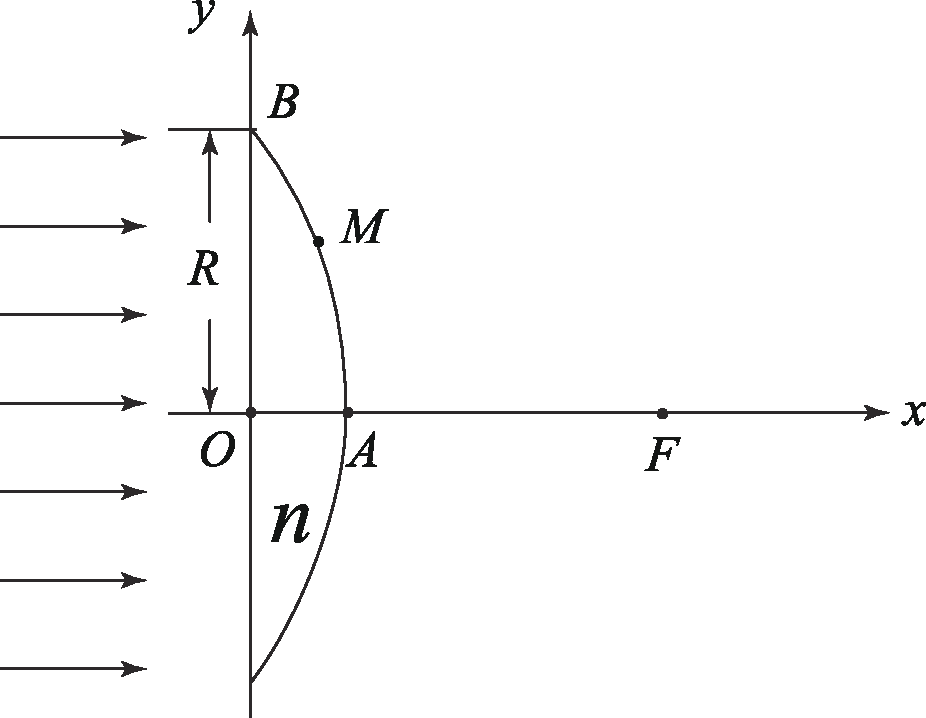
\includegraphics[width = 0.4\textwidth]{images/opt-8.pdf} 
		\end{flushright}
	
	\tagged{student}{\vspace*{2cm}}
	\begin{taggedblock}{teacher}
		\noindent
		解析:
			\begin{figure}[hbtp]
					\includegraphics[width = 0.3\textwidth]{images/opt-6-5.pdf} 
				\end{figure}
		\\1.$x_0=\frac{n\sqrt{f'^2+R^2}-f'}{n^2-1},a=\frac{nf'-\sqrt{f'^2+R^2}}{n^2-1}$,$(n^2-1)(x-x_0)^2-y^2=a^2$ 旋转双曲面
		\\2.透镜顶点A的位置满足:$(n^2-1)(x_A-x_0)^2=a^2$ 或者$x_A=x_0-\frac{a}{\sqrt{n^2-1}}=\frac{\sqrt{f'^2+R^2}-f'}{n-1}$
		\\3.$x_A\leq f'$,得出$\frac{\sqrt{f'^2+R^2}-f'}{n-1}\leq f'$
	\end{taggedblock}
\end{example}
%%%%%%%%%%%%%%%%%%%%

%%%%%%%%%%%%%%%%%%%%%%%%%%%%%%%%%%%%%%%%%%%%%%%%%%%%%%%%%%%%%%%%%%%%%%%%%%%%
\section{近轴成像}

从前面的例子可以看出,那些具有理想光学性质的光学仪器一般具有非常复杂的形状,使得它们难以加工或成本极高。
反过来那些具有简单形状的光学界面则容易生产,但是它们的光学性质却并不是十分理想。
理论和经验都表明,如果入射光线非常接近于光学系统的对称轴,具有简单形状的光学仪器依然能在相当的满意程度上成像。
与光学系统的主对称轴偏离不大的光线称为近轴光线,很明显近轴光线与主光轴的夹角不会太大,对于它们的处理可以利用一些合理的近似以简单计算,本节就来关注近轴光线的近似性质以及它们成像的特点。

在折射定律\ref{eqn: geo-refraction law}当中,如果入射光和折射光与法线的夹角很小时,它们的正弦值与弧度值之间的差别很小,在这样的近似下折射定律被简化为入射角与反射角的比值为一常数\footnote{在人们研究折射现象的早期一直认为真实的折射定律就是取这样的正比,但随后发现在大的折射角度下与它的偏离比较大,随后才得到正确的基于正弦值的折射定律}:
\begin{equation}
\frac{\alpha}{\beta}=n,\qquad \alpha = n\beta
\end{equation}

\begin{example}
水面下方深度为$h$处有一个物体$A$,求位于该物体正上方与水面距离为$d$附近的观察者所看到的物体的位置。
已知水的折射率为$n$,忽略空气与真空折射率的差别。

\begin{flushright}
\includegraphics[width = 0.3\textwidth]{images/depth-look.pdf}
\end{flushright}
\tagged{student}{\vspace*{0cm}}
\begin{taggedblock}{teacher}

\includegraphics[width = 0.4\textwidth]{images/depth-look-solution.pdf}
\newline
解析:如图所示,做一条近轴光线以及它的法线,为了直观图中将光线画得偏了一些,实际上它非常接近于AB的连线。
根据折射定律的小角度近似$n\alpha = \beta$。
在图中也把由几何关系决定了的其它量标记了出来,今线段SP的长度为$l$,注意它是一个很短的长度。

由几何关系我们有$h\alpha = l$以及$h'\beta = l$,将它们两式联立可得
\[
h' = \frac{1}{n}h
\]
这样从B点看到的物体的像与它的距离就是$d+\frac{1}{n}h$。
这个关系在研究成像过程当中非常有用。
从中还可以看出一般性的结论:从折射率为$n$的介质射向真空,视深度缩小$n$倍,反之从真空(空气)射向介质,视深度增加$n$倍。
\end{taggedblock}
\end{example}


\begin{example}
如图得示有一个半径为$R$的球面反射镜,在它对称轴上与顶点相距$u$处有一个发光点($u>R$),它发出的光被位于光轴的一个光圈限制,使得只有近轴光线才能够被球面镜反射。
求证在近轴近似下所有的光线将会聚到光轴上的一点$B$,并给出$B$点与球面镜顶点的距离$v$。

\begin{flushright}
\includegraphics[width=0.3\textwidth]{images/sphrical-mirrow.pdf}
\end{flushright}
\tagged{student}{\vspace*{0cm}}
\begin{taggedblock}{teacher}



\noindent
解析:考虑如图所示的近轴光线,设它与光轴的夹角为$\beta$,在入射点$P$处的入射角为$\alpha$,其它有关的角度可由几何关系导出。
它们都是很小的角度,也就是说它们的弧度值、正弦值与正切值之间近似认为没有差别。
除此之外在长度方面也有一些重要的近似,例如图中AP线段的长度与物距$u$的差别就非常之小,可以忽略不计,同样的道理BP的长度与像距$v$也可做相等的近似。
\includegraphics[width=7cm]{images/sphrical-mirrow-solution}

在三角形AOP当中使用正弦定理,并利用前面提到的近似可以得到
\[
\frac{u-R}{\alpha}=\frac{u}{\alpha+\beta}
\]
同理在三角形OPB当中有
\[
\frac{R-v}{\alpha}=\frac{v}{\alpha+\beta}
\]
两式相比,消去所有的角度可得
\[
\frac{u-R}{R-v}=\frac{u}{v}
\]
从中可以看出像距$v$在近轴近似下与光线的倾角$\beta$无关,可知所有的近轴光线经过球面镜反射以后能够会聚到一点。
化简以后可以得到$u$、$v$和$R$之间更对称的关系
\[\frac{1}{u}+\frac{1}{v}=\frac{2}{R}\]
用类似的方法其实还可以得到其它位置的成像关系,经过总结就可以得出球面镜近轴成像的公式。

除了几何方法,还可以用等光程的条件来决定像的位置。
对于给定的物距$u$,设像距为$v$,它现在是一个未知数。
在球面上取与主光轴非常接近的一点$P$,它与球心的连线与光轴的夹角设为$\theta$。
这样由$A$经过$P$点到达像点$B$的光程为
\[
S = \sqrt{(u-R)^2+R^2+2u(u-R)\cos\theta}+\sqrt{(R-v)^2+R^2+2R(R-v)\cos\theta}
\]
如果光线能够会聚到B点,要求上式给出的光程相对于$\theta$角的变化对于近轴光线,也就是$\theta=0$附近为稳定值,将$S$对$\theta$求导
\[
\frac{dS}{d\theta}(\theta = 0) = \frac{R(u-R)}{u}\sin\theta -\frac{R(R-v)}{v}\sin\theta=0 
\]
将它整理同样可得和前面一样的成像公式。
\end{taggedblock}
\end{example}


\begin{example}
	如图所示,一细长的圆柱形均匀玻璃棒,其一个端面是平面(垂直于轴线),另一个端面是球面,球心位于轴线上。
	现有一很细的光束沿平行于轴线方向且很靠近轴线人射,当光从平端面射人棒内时,光线从另一端面射出后与轴线的交点到球面的距离为$ a$;当光线从球形端面射人棒内时,光线在棒内与轴线的交点到球面的距离为$b$。试近似地求出玻璃的折射率$ n$。
	\begin{flushright}
		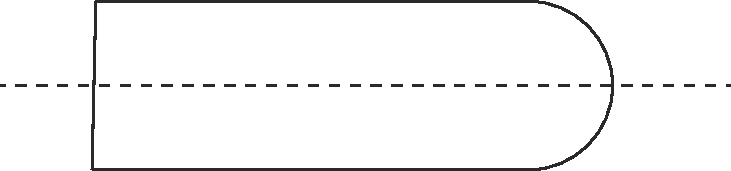
\includegraphics[width = 0.4\textwidth]{images/opt-9.pdf} 
	\end{flushright}
	\tagged{student}{\vspace*{1cm}}
	\begin{taggedblock}{teacher}
		\noindent
		解析:$n=\frac{b}{a}$
	\end{taggedblock}
\end{example}

\begin{example}
有一个球心位于$O$点、顶点位于$S$点半径为$R$的球形表面,其左侧为真空,右侧充满折射率为$n$的均匀介质,$SO$位于主光轴上。
对于主光轴上$S$点左侧与其相距$u$处有一发光点$A$,求证$A$点发出的近轴光线经过折射以后全部会聚于主光轴上的某点$B$,并求出$B$与顶点$S$的距离$v$。

在最简单的情况下人眼可以看成是一个折射率$n=4/3$,半径$R=5.56\unit{mm}$的球体,这个模型称为简约眼,求在近轴近似下平行光经过简约眼折射以后能够会聚到角膜后方何处?
\begin{flushright}
\includegraphics[width = 0.4\textwidth]{images/sphrical-lense.pdf}
\end{flushright}
\tagged{student}{\vspace*{1cm}}
\begin{taggedblock}{teacher}
\noindent
解析:如问题当中的图所示,设入射角为$\alpha$,折射角为$\beta$,根据题目假设我们知道它是一条近轴光线,所以两个角度均为小角,可应用小角度近似,这样折射定律变成了$\alpha=n\beta$。
再令入射光与光轴的夹角为小角$\gamma$,近轴近似下我们还有$AP\simeq u$和$BP\simeq v$。

在三角形APO当中使用正弦定理并利用这些近似可得
\[
\frac{u}{\alpha-\gamma}=\frac{u+R}{\alpha}
\]
同样在三角形BPO当中有
\[
\frac{v}{\alpha-\gamma}=\frac{v-R}{\beta}
\]
两式相比并利用折射定律可得
\[  \frac{u}{v}=\frac{1}{n}\cdot\frac{u+R}{v-R}\]
和球面镜一样,近轴近似下球形表面折射后像点的位置与角度$\gamma$无关,说明它们能够会聚到同一点。
化简上式可以得到像点的位置与其它量所满足的关系:
\[
\frac{1}{u}+\frac{n}{v}=\frac{n-1}{R}
\]

平行光可看成是位于$u=\infty$处物体所发出的光,对于简约眼将$u=\infty$代入上式可得
\[
v=\frac{n}{n-1}R=22.24\unit{mm}
\]
\end{taggedblock}
\end{example}



\section{常见成像系统与符号法则}

在近轴近似下那些具有简单形状、易于制造的光学仪器同样具有较好的光学性质,我们可以利用这些光学性质用来改变光路使人们看到那些肉眼不无看到的对象。
在研究真实的光学仪器之前,有必要整理一下光学系统成像的一般性质,并熟悉几个新的术语。
最理想的情况下从一点$A$发出的光线通过光学系统的折射、反射以后能够或在近轴近似下能够会聚到$B$点,就称$A$为{\heiti 物}(object),$B$为{\heiti 像}(image)。注意一次成像过程下的像也可以作为下一次成像过程的物。

对于实际的情况,通过光学系统以后有可能形成发散光,这些光线不可能会聚到一点,但是它们的反向沿长线能够会聚到一点上,这时我们称其为{\heiti 虚像}(virtual image),与之相对应的,那些由真实光线会聚形成的像称为\emph{实像}(real image)。
虚像和实像有一个重要的区别,只需要注意到光具有能量,只有实像处才会有能量聚集\footnote{当然一个实像也可以因为在光线未聚焦前进入另一个光学仪器而未被展现出来},可以通过屏或其它感光元件收集光信号,虚像则不同,只能通过肉眼或拍摄装置来观测。

对于物来说也有两种不同的情况,如果通过光学仪器的光线是从一点发出的光,就称这个物为{\heiti 实物}(real subject)
除此之外还有另外一种可能性,例如有一束会聚到一点的光,但在它们没有会聚之前就遇到了一个光学设备,这时光线就需要立刻折射或反射,在这种情况下就称那个将要会聚的点为本次成像过程的{\heiti 虚物}(virtual subject)。

像和物都有虚实之分,所以在分析成像过程一定要密切注意到这一点。

除了像的位置,有时候还会关注像的大小,对于球面镜来说可以很容易地证明,在近轴光线成像的近似下像与物大小的比值就等于像距与物距的比值的绝对值,无论物与像的虚实这一关系都成立,对于一次成像过程,定义其放大率
\begin{equation}
S = -\frac{y^\prime}{y}
\end{equation}
特别需要注意的是放大率与人眼看上去物体变大多少是不一样的,人眼所看到物体的大小不但依赖于物体本身的大小,还和它与眼睛的距离有关,也就是人们常说的“近大远小”的道理。

如图凸透镜,它有一条对称轴,称为{\heiti 主光轴},主光轴上有对称分布的两个点$F$和$F'$,称为凸透镜的{\heiti 焦点},它们与透镜中心的距离称为{\heiti 焦距},通过焦点垂直于主光轴的平面称为\emph{焦平面}。
从一点发出的光经过凸透镜都能会聚到另一点上,并且具有三条容易决定的特殊光线:
\begin{enumerate}
\item 平行于主光轴的入射光线经凸透镜折射以后变成通过其焦点。
\item 通过凸透镜中心的光线方向不变
\item 通过一侧焦点的入射光经过透镜变成平行于主光轴
\end{enumerate}
对于凹透镜和凸透镜稍有不同,通过凹透镜中心的光线依然不改变方向,但是平行于光轴的光经过凹透镜折射以后变成其反向沿长线通过同侧焦点的光;其沿长线通过对侧焦点的光则变成平行光。
由于凹透镜是发散透镜所以在通常情况下它无法对实物成实像,但是这些光线的反向沿长线却交于一点,可以成一个正立的虚像。






\section{球面镜、透镜成像}
以透镜为例,图\ref{fig: geo-lense-various-case}给出了透镜成像的四种典型的情况,对于面镜来说也是类似的,请同学们自己将它们画出。
\begin{figure}
\begin{center}
\includegraphics[width=0.9\textwidth]{images/lense-various-case.pdf}
\caption{透镜成像的各种可能性:(1)实物成实像,(2)实物成虚像,(3)虚物成实像,(4)虚物成虚像}
\label{fig: geo-lense-various-case}
\end{center}
\end{figure}



\begin{example}
请证明:无论物与像的虚实,反射面的凹凸,近轴近似下{\heiti 球面镜}(spherical mirror)的成像公式均为$\frac{1}{u}+\frac{1}{v}=\frac{2}{R}$,其中各个量的正负号定义如下:
\begin{itemize}
\item 物距:实物$u>0$,虚物$u<0$
\item 像距:实像$v>0$,虚像$v<0$
\item 半径:凹面镜$R>0$,凸面镜$R<0$
\end{itemize}

\tagged{student}{\vspace*{3cm}}
\begin{taggedblock}{teacher}
\noindent
解析:略
\end{taggedblock}
\end{example}



%%%%%%%%%%%%%
\begin{example}
	图中$L$为一薄凸透镜,$ab$为一发光圆面,二者共轴,$S$为与$L$平行放置的屏。
	已知这时$ab$可在屏上成清晰的像。
	现将透镜切除一半,只保留主轴以上的一半透镜,请分析$ab$在$S$上的像尺寸、形状和亮度的变化。
		\begin{flushright}
			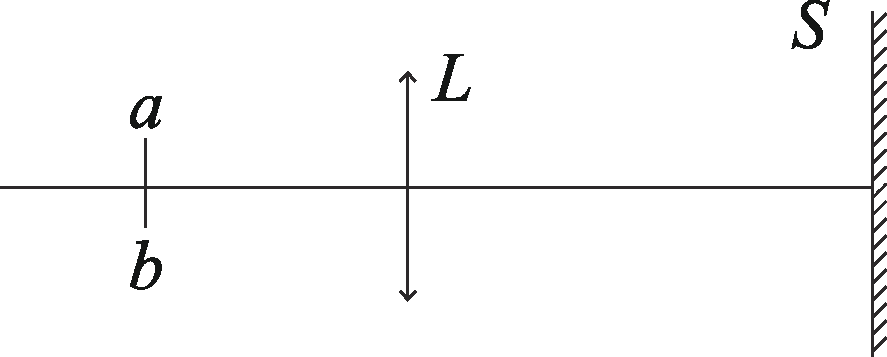
\includegraphics[width = 0.4\textwidth]{images/opt-18.pdf} 
		\end{flushright}
	\tagged{student}{\vspace*{1cm}}
	\begin{taggedblock}{teacher}
		\noindent
		解析:尺寸、形状不变,亮度变暗
	\end{taggedblock}
\end{example}
%%%%%%%%%%%%%%%%%%%%

\begin{example}
	在焦距为$f$的凸透镜主光轴上有一个运动光源,当光源位于何处时像的移动速度与光源的速度相同?
	\tagged{student}{\vspace*{3cm}}
	\begin{taggedblock}{teacher}
		\newline
		解析:当物距为$u$时根据成像公式像距
		\[
		v=\frac{fu}{u-f}
		\]
		设运动光源的运动速度$V_O = \frac{du}{dt}$,根据链式法则像的运动速度
		\[
		V_I = \frac{dv}{dt}=-\frac{f^2}{(u-f)^2}\frac{du}{dt}
		\]
		式中的负号是由物距和像距的定义方式带来的,像速度与物速度相同要求$f=u-f$,很明显当物体处于二倍焦距处时两者的速度相同
	\end{taggedblock}
\end{example}


%%%%%%%%%%%%%
\begin{example}
	光源位于$f'=30\si{mm}$的透镜前 40mm 处,问屏放在何处能找到光源像?垂轴放大率等于多少?若光源及屏位置保持不变,问透镜移到什么位置时,能在屏上重新获得光源像,此时放大率等于多少?
	\tagged{student}{\vspace*{4cm}}
	\begin{taggedblock}{teacher}
		\newline
		解析:120mm处,放大率为3;远离光源移动80mm,放大率为$\frac{1}{3}$
	\end{taggedblock}
\end{example}
%%%%%%%%%%%%%%%%%%%%

%%%%%%%%%%%%%
\begin{example}
水平放置的曲率半径$ R=60$cm 的凹球面镜装有水,水的折射率是 1.333,假设水的深度比半径$ R $要小得多,试求它的焦距?
	\tagged{student}{\vspace*{4cm}}
	\begin{taggedblock}{teacher}
		\newline
		解析:$f=\frac{R}{n-1}$
	\end{taggedblock}
\end{example}
%%%%%%%%%%%%%%%%%%%%

%%%%%%%%%%%%%
\begin{example}
如图所示为一凹球面镜,球心为$ C$,内盛透明液体。已知$ C $至液面高度$ CE $为 $40.0$cm,主轴$ CO $上 有一物$A$,物离液面高度$AE$恰好为$ 30.0$cm 时,物$A $的实像和物处于同一高度。实验时光圈直径很小,可以保证近轴光线成像。试求该透明液体的折射率$ n$。
	\begin{flushright}
		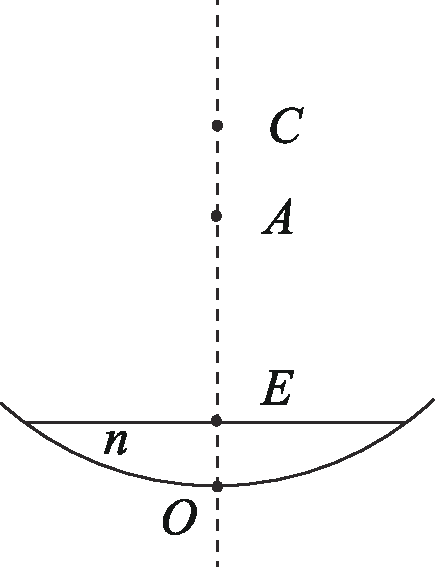
\includegraphics[width = 0.3\textwidth]{images/opt-10.pdf} 
	\end{flushright}
	\tagged{student}{\vspace*{1cm}}
	\begin{taggedblock}{teacher}
		\noindent
		解析:n=1.33
	\end{taggedblock}
\end{example}
%%%%%%%%%%%%%%%%%%%%




\begin{figure}
\begin{center}
\includegraphics[width = 0.9\textwidth]{images/lense-tu-path.pdf}
\end{center}
\end{figure}
和球面镜成像公式相类似的还有透镜的情况,与反射镜不同的是利用光的折射改变光路的透镜必然有一定的厚度。
这里我们首先忽略透镜的厚度,称其为{\heiti 薄透镜}(thin lens),并对它的光学性质做一些理想化的假设。


通过三条特殊的光路可以在一般情况下在给定物的位置和大小以后求出像的位置和大小,请同学们自行证明理想{\heiti 球透镜}(spherical lens)的成像公式为
\begin{equation}
\frac{1}{u}+\frac{1}{v}=\frac{1}{f}
\end{equation}
其中$u$、$v$和$f$分别代表物距、像距和透镜焦距。
和球面镜类似,放大率也是像距和物距之比:
\begin{equation}
S = \left |\frac{v}{u}\right |
\end{equation}
和球面镜类似,成像定律当中$u>0$代表实物,$u<0$代表虚物,$v>0$代表实像,$v<0$代表虚像,$f>0$代表凸透镜,$f<0$代表凹透镜。

\begin{example}
物位于凸透镜左边的不同位置,根据凸透镜成像和放大率的公式以及光路定性地分析凸透镜成像的性质并完成下表。
感兴趣的同学还可以完成对于凹透镜和凹凸球面镜类似的表格。

\begin{tabular}{|c|c|c|c|c|}
\hline 
物距 & 左侧或右侧 & 正立或倒立 & 实像或虚像 & 放大或缩小 \\ 
\hline 
$\infty>u>2f$ &  &  &  &  \\ 
\hline 
$2f>u>f$ &  &  &  &  \\ 
\hline 
$f>u>0$ &  &  &  &  \\ 
\hline 
虚物 $u<0$ &  &  & &  \\ 
\hline 
\end{tabular} 
\tagged{student}{}
\begin{taggedblock}{teacher}
\newline
解析:略
\end{taggedblock}
\end{example}




%\begin{example}
%给定曲面形状决定焦距
%\tagged{student}{\vspace*{4cm}}
%\begin{taggedblock}{teacher}
%\newline%
%解析:
%\end{taggedblock}
%\end{example}



\section{光具组成像}
当把多个透镜或反射镜放在一起时,光线会依次通过各个透镜或反射镜,受它们的影响传播方向会发生变化。
前面我们分析了单个透镜或球面镜的成像规律,把它们放在一起时只需要沿着光传播的方向依次对于每个光学器件应用成像公式求出单次成像的位置、大小、虚实等相关物理量,并且注意到前一个光具的像就是后一个光具的物,连续使用成像公式就能够得到最终像的各种信息。
由于各个镜摆放位置各有不同,要注意前一个镜的虚像并不一定意味着就是后一个镜的虚物,同理实像也不一定意味着实物,对于单个透镜来说像或物的虚实只取决于入射光本身的性质。


\begin{example}
	试证明两个紧贴在一起焦距分别为$f_1$和$f_2$的薄透镜的成像效果和一个焦距满足
	\[\frac{1}{f}=\frac{1}{f_1}+\frac{1}{f_2}\]
	的理想透镜完全一致。
	\tagged{student}{\vspace*{3cm}}
	\begin{taggedblock}{teacher}
		\newline
		解析:设对于前一个透镜物距为$u_1$,通过第一个透镜成像的像距
		\[
		\frac{1}{u_1}+\frac{1}{v_1}=\frac{1}{f_1},
		\]
		对于第二个透镜来说,当$v_1>0$时第一个透镜的像是一个虚物$u_2=-v_1$,当$v_1<0$时第一个透镜的像是一个实物$u_2=-v_1$,无论哪种情况我们都有对第二个透镜来说$u_2=-v_1$。
		对第二个透镜应用成像公式,设像距为$v_2$,可得
		\[
		\frac{1}{u_2}+\frac{1}{v_2}=-\frac{1}{v_1}+\frac{1}{v_2}=\frac{1}{f_2}
		\]
		两个成像公式相加有
		\[\frac{1}{u_1}+\frac{1}{v_2}=\frac{1}{f_1}+\frac{1}{f_2}\]
		比单个透镜的成像公式相比较可以得出结论。
		
		
		
	\end{taggedblock}
\end{example}


%%%%%%%%%%%%%
\begin{example}
	一平凸透镜焦距为$f$,其平面上镀了银,现在其凸面一侧距它$ 2f$处,垂直于主轴放置一高为$H$的物, 其下端在透镜的主轴上。
	
	(1)用作图法画出物经镀银透镜所成的像,并标明该像是虚、是实。 
	
	(2)用计算法求出此像的位置和大小。
	
	\begin{flushright}
		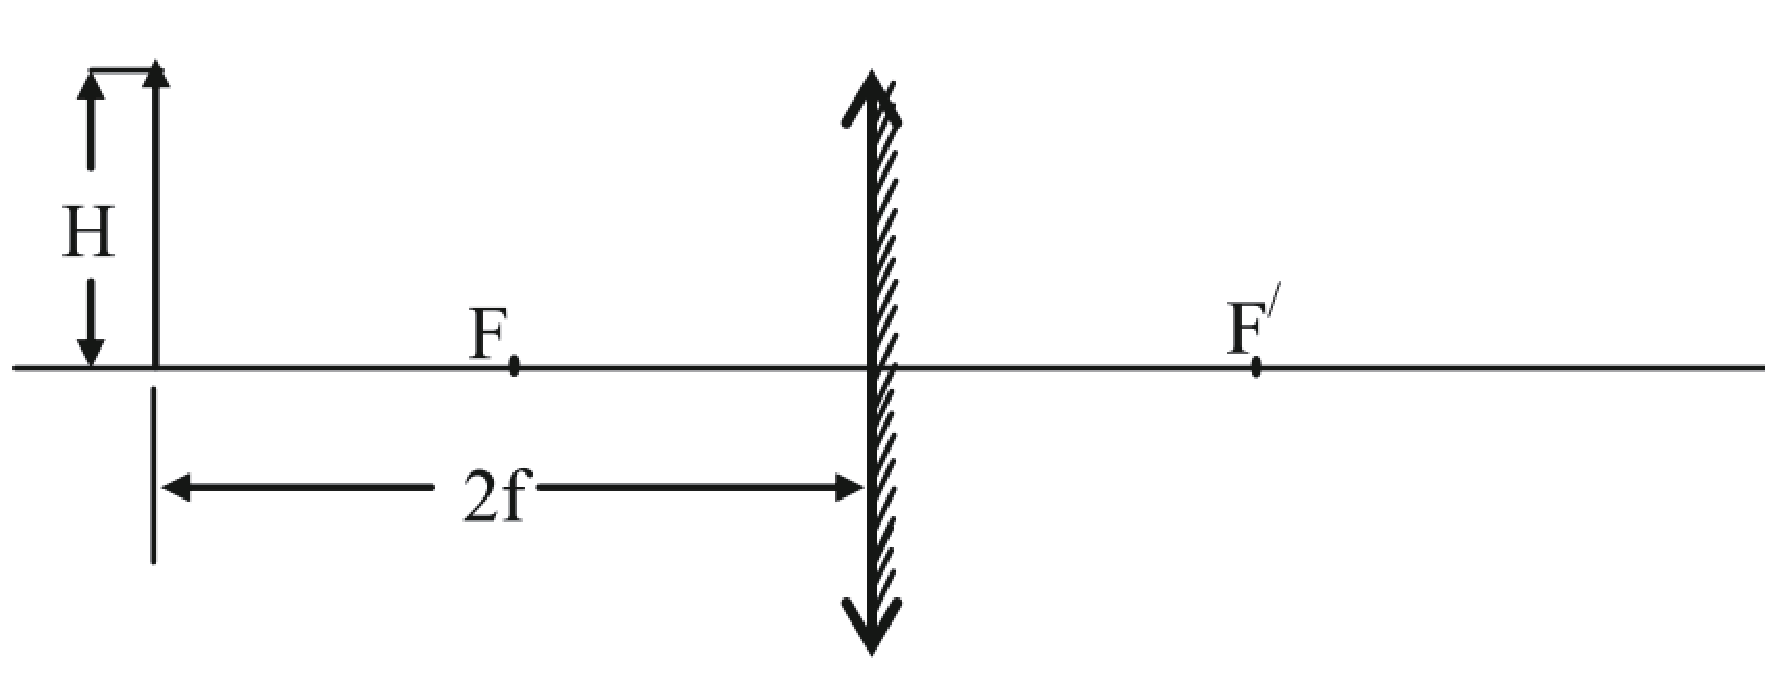
\includegraphics[width = 0.4\textwidth]{images/opt-11.pdf} 
	\end{flushright}
	
	\tagged{student}{\vspace*{4cm}}
	\begin{taggedblock}{teacher}
		\noindent
		解析:\begin{figure}
							\includegraphics[width = 0.5\textwidth]{images/opt-10-5.pdf} 
						\end{figure}
				\\作图法:平凸透镜平面上镀银后构成一个由会聚透镜L和与它密接的平面镜M组合LM,如图所示。图中O为L的光心, 为主轴,F和 为L的两个焦点,AP为物。作图时利用了下列三条特征光线:
				\\①由P射向O的入射光线,它通过O后方向不变,沿原方向射向平面镜M,然后被M反射,反射光线与主光轴的夹角等于入射角,均为$\alpha$。反射线射入透镜时通过光心O,故由透镜射出时方向与上述反射线相同,即图中的$OP'$ 。
				\\②由P发出且通过L左方焦点F的入射光线PFR,它经过L折射后的出射线与主轴平行,垂直射向平面镜M,然后被M反射,反射光线平行于L的主轴,并向左射入L,经L折射后的出射线通过焦点F,即为图个中RFP。
				\\③由P发出的平行于主轴的入射光线PQ,它经过L折射后的出射线将射向L的焦点 ,即沿图中的 方向射向平面镜,然后被M反射,反射线指向与 对称的F点,即沿QF方向。此反射线经L折射后的出射线可用下法画出:通过O作平行于QF辅助线 , 通过光心,其方向保持不变,与焦面相交于T点。由于入射平行光线经透镜后相交于焦面上的同一点,故QF经L折射后的出射线也通过T点,图中的QT即为QF经L折射后的出射光线。
				上列三条出射光线的交点 即为LM组合所成的P点的像,对应的 即A的像点。由图可判明,像 是倒立实像,只要采取此三条光线中任意两条即可得 ,即为正确的答案。
				\\
				\\计算法:透镜左方距离$\frac{3}{2}f$处,像高为物高的$\frac{1}{3}$                                                                                                                                                                          
	\end{taggedblock}
\end{example}
%%%%%%%%%%%%%%%%%%%%


%%%%%%%%%%%%%
\begin{example}
	如图所示,折射率$ n=1.5 $的全反射棱镜上方 6cm处放置一物体$AB$,棱镜直角边长为 6cm,棱镜右侧 10cm处放置一焦距$ f_1=10$cm 的凸透镜,透镜右侧 15cm处再放置一焦距$ f_2=$10cm的凹透镜,求该光学系统成的位置和像放大率。
		\begin{flushright}
			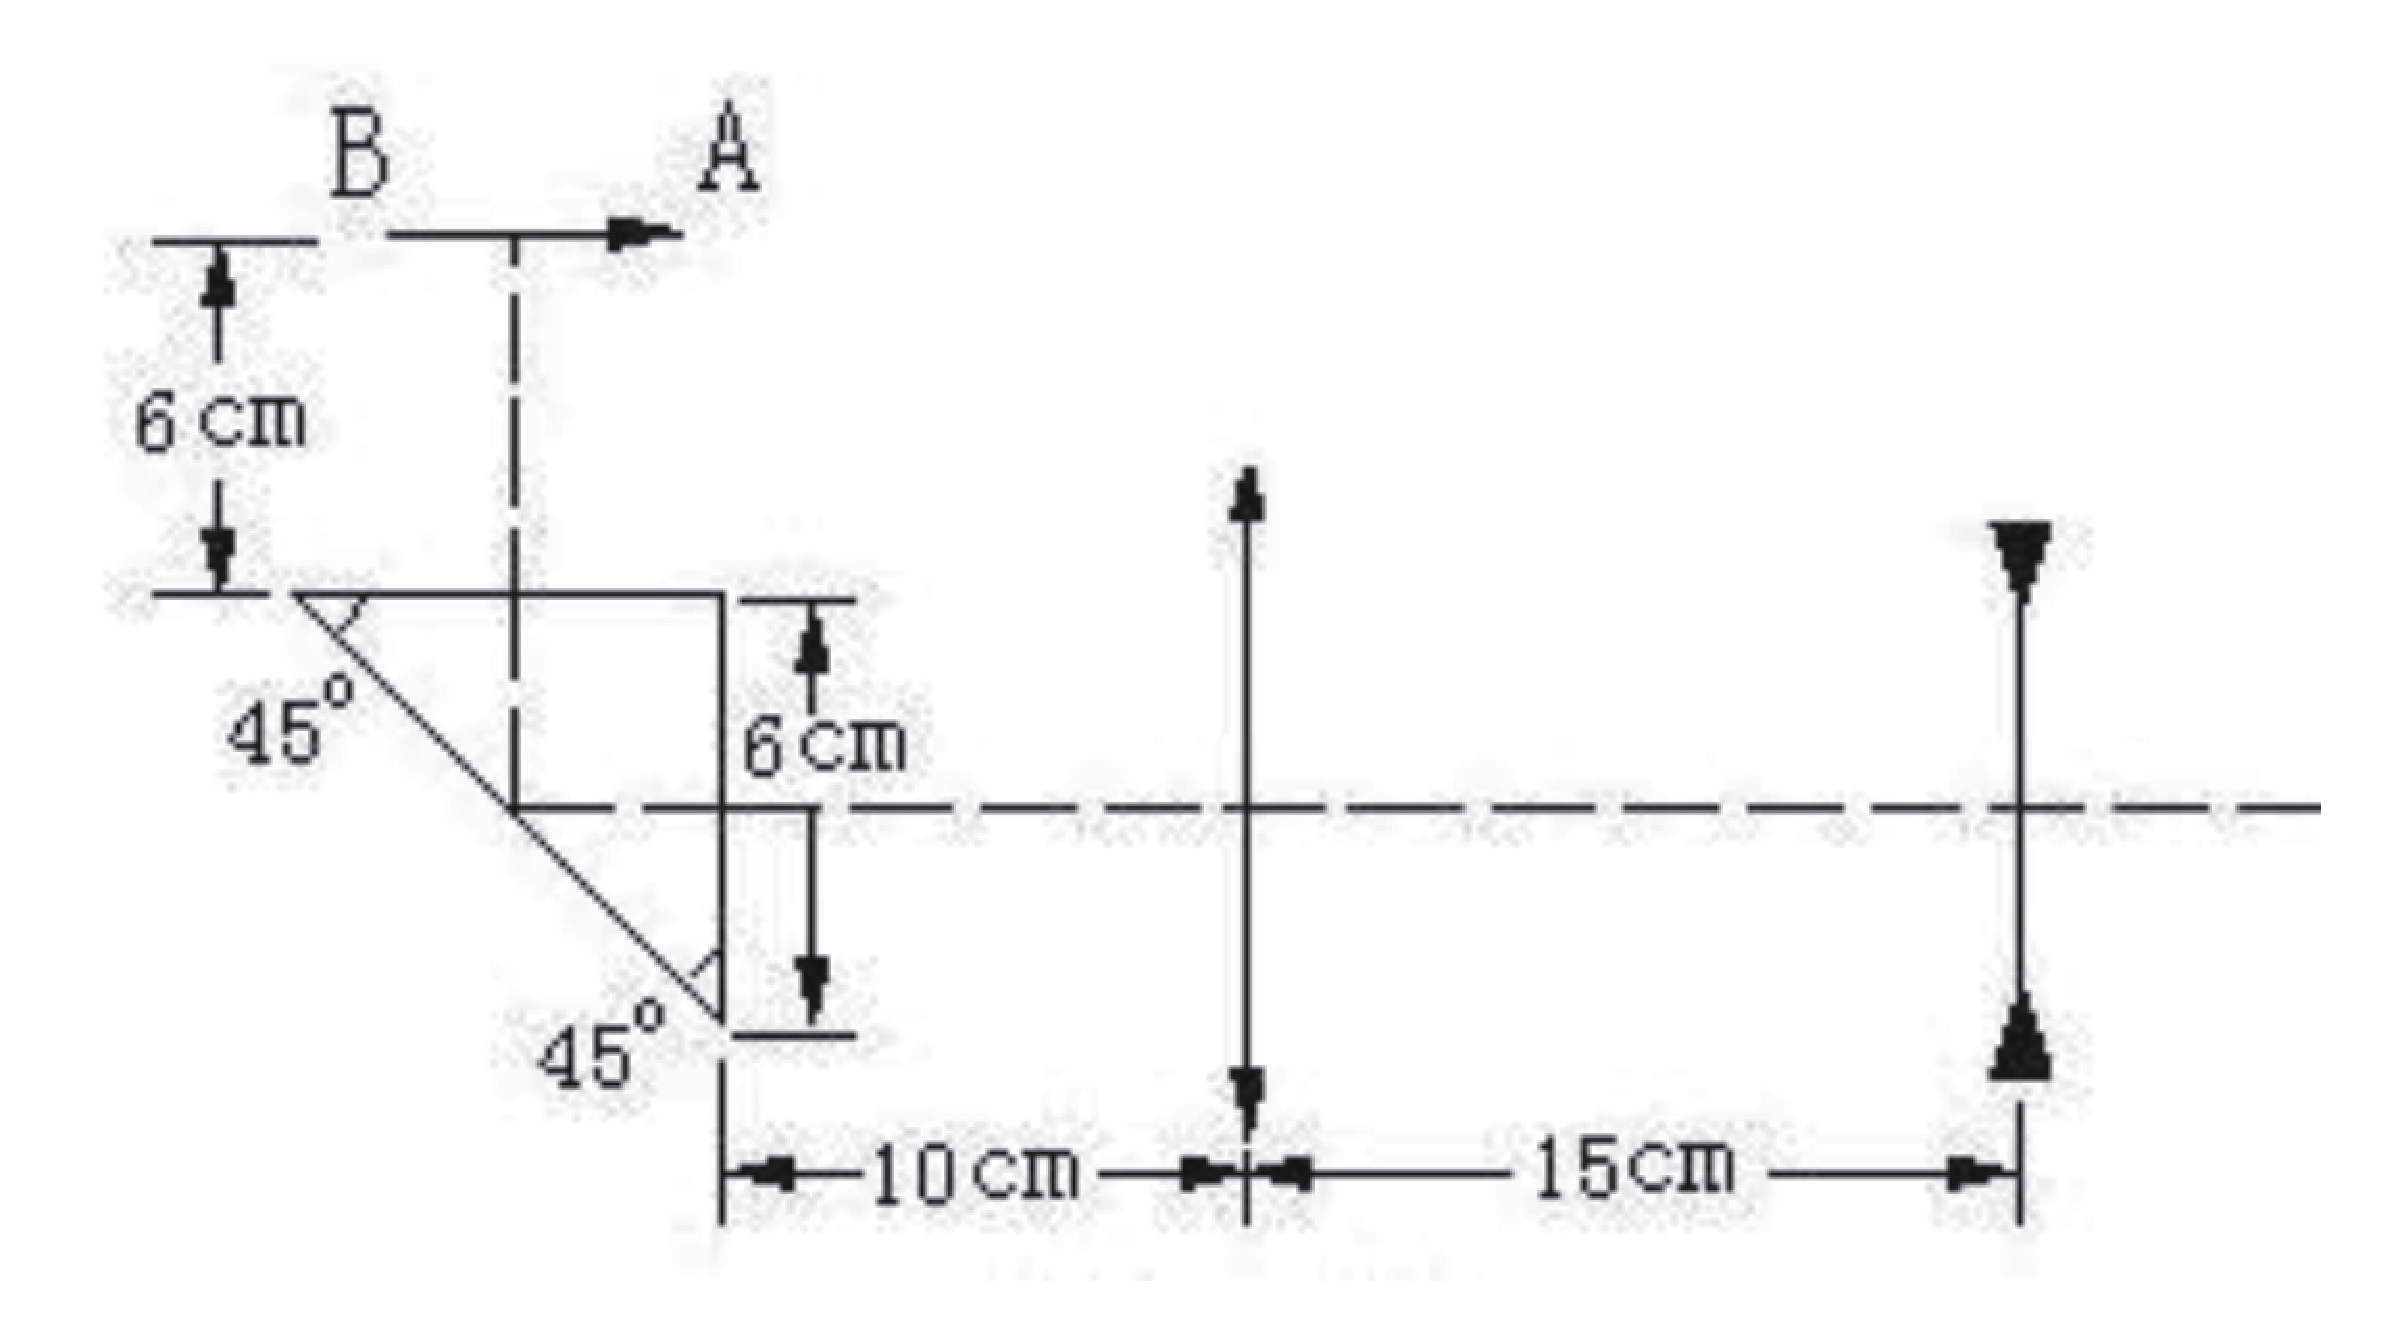
\includegraphics[width = 0.5\textwidth]{images/opt-13.pdf} 
		\end{flushright}
	\tagged{student}{\vspace*{4cm}}
	\begin{taggedblock}{teacher}
		\noindent
		解析:在凹透镜右侧10cm,实相,放大率2
	\end{taggedblock}
\end{example}
%%%%%%%%%%%%%%%%%%%%



%%%%%%%%%%%%%
\begin{example}
如图所示,$L $是一焦距为$ f$的薄凸透镜($F$与$ F'$为其焦点).在透镜右侧焦
	点$ F'$处放置一曲率半径大小为$R $的球圈反射镜(其顶点位于$ F'$处),透镜和球面组成一轴对称的光学系统,在透镜$ L $左侧光轴上有限远处有一发光点$ P$,它发出的傍轴光线经此光学系统后,恰好成像在$P $点。
	
	1. 若球面镜为凹面镜,则$P $点到透镜的距离等于\kong;若球面镜为凸面镜,则$P$ 点到透镜的距离等于\kong。
	
	2.若将一短细杆垂直于光轴放置,杆的下端位于$ P$点,则此细杆经上述光学系统所成	的最后的像的大小与物的大小之比对凹透镜等于\kong;对凸透镜等于 \kong.
	
	3.若球面镜子半径大小$ R=2f$,试按作图法的规范要求,画出第 2 问中短杆对上述光学系统逐次成的像及成像光路图.
	
	\begin{center}
		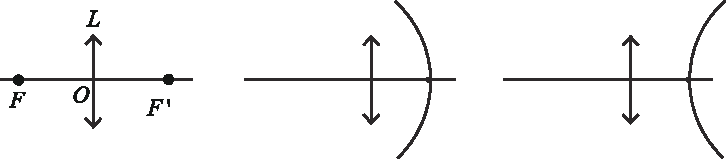
\includegraphics[width=0.95\textwidth]{images/opt-17.pdf}
	\end{center}
	\tagged{student}{\vspace*{4cm}}
	\begin{taggedblock}{teacher}
		\noindent
		解析:1.$\frac{f(R-f)}{R},\frac{f(R+f)}{R}$
		\\2.1;1
		\\3.略
	\end{taggedblock}
\end{example}
%%%%%%%%%%%%%%%%%%%%



\begin{example}
如图所示,$L$是一个焦距为$2R$的薄凸透镜,$MN$为其主光轴。
在$L$的右侧与它共轴地放置两个半径都为$R$的很薄的球面镜$A$和$B$。
每个球面镜的凹面和凸面都是能反光的镜面。
$A$、$B$顶点间的距离为$\frac{3}{2}R$,在$B$的顶点$C$处开有一个透光的小圆孔(圆心为$C$),圆孔的直径为$h$。
现于凸透镜$L$左方距$L$为$6R$处放一个与主轴垂直的高度也为$h$($h\ll R$)的细短杆$PQ$($P$在主轴上),$PQ$发出的光经$L$后其中一部分穿过$B$上的小圆孔正好成像在球面镜$A$的顶点$D$处,形成物$PQ$的像$I$。求

\begin{center}
\includegraphics[width=0.7\textwidth]{images/lense-comples-problem.pdf}
\end{center}


1. 像$I$与透镜$L$的距离等于\underline{$\qquad$}。

2. 形成像$I$的光线经$A$反射,直接通过小孔后经$L$所成的像$I_1$与透镜$L$的距离等于\underline{$\qquad$}。

3. 形成像$I$的光线经过$A$反射,再经$B$反射,再经$A$反射,最后通过$L$成像为$I_2$,将$I_2$的有关信息填在下表中:

\begin{tabular}{|c|c|c|c|c|}
\hline 
与$L$的距离 & 在$L$的左或右 & 大小 & 正立/倒立 & 实像/虚像 \\ 
\hline 
 &  &  &  &  \\ 
\hline 
\end{tabular} 

4. $PQ$发出的光经$L$后未进入$B$上小圆孔$C$的那一部分光最后通过$L$成像为$I_3$,将$I_3$的有关信息填在下表中:

\begin{tabular}{|c|c|c|c|c|}
\hline 
与$L$的距离 & 在$L$的左或右 & 大小 & 正立/倒立 & 实像/虚像 \\ 
\hline 
 &  &  &  &  \\ 
\hline 
\end{tabular} 

\tagged{student}{\vspace*{4cm}}
\begin{taggedblock}{teacher}
\noindent
解析:1.3R;
\\2.6R;
\\3.6R、右方、2h、倒立、虚像;
\\4.18R、左方、1.8h、正立、实像.
\end{taggedblock}
\end{example}





\begin{example}
图中$L_1$为一薄凸透镜,Q为高$2.00\unit{cm}$、与光轴垂直放置的线状物,已知$Q$经$L_1$成一实像,像距为$40.0\unit{cm}$。
现于$L_1$的右方依次放置凹透镜$L_2$,$L_3$和薄凸透镜$L_4$以及屏$P$,它们之间的距离如图所示。
所有的透镜都共轴,屏与像垂直,$L_2$、$L_3$的焦距大小均为$15\unit{cm}$。
已知物$Q$经上述四个透镜最后在屏上成倒立的实像,像高为$0.500\unit{cm}$。
求$L_1$和$L_4$的焦距。
\begin{flushright}
\includegraphics[width=0.6\textwidth]{images/lense-group-problem.pdf}
\end{flushright}
\tagged{student}{\vspace*{4cm}}
\begin{taggedblock}{teacher}
\noindent
解析:$L_1:19.2(19.0-19.4)$  $L_2:10.2(10.0-10.4)$
\end{taggedblock}
\end{example}



%%%%%%%%%%%%%
\begin{example}
	薄凸透镜放在空气中时,两侧焦点与透镜中心的距离相等。如果此薄透镜两侧的介质不同,其折射率分别为$n_1$和$n_2$,则透镜两侧各有一个焦点(设为$F_1$和$F_2$ ),但$F_1$、$F_2$和透镜中心的距离不相等,其值分别为$f_1$和$f_2 $。现有一个薄凸透镜$L$,已知此凸透镜对平行光束起会聚作用,在其左右两侧介质的折射率及焦点的位置如图所示。 
	
	1.试求出此时物距$u$,像距$v$,焦距$f_1$、$f_2 $四者之间的关系式。 
	
	2.若有一傍轴光线射向透镜中心,已知它与透镜主轴的夹角为$\theta_1$,则与之相应的出射线与主轴的夹角$\theta_2$多大? 
	
	3. $f_1,f_2,n_1,n_2$四者之间有何关系?
	
		\begin{flushright}
			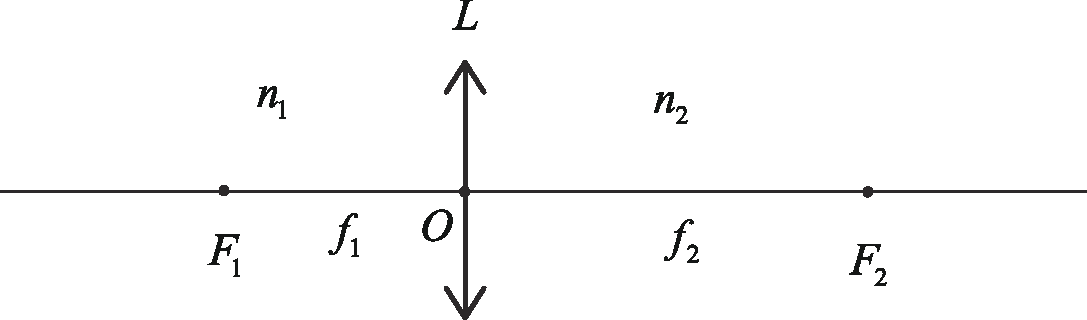
\includegraphics[width = 0.5\textwidth]{images/opt-14.pdf} 
		\end{flushright}
	\tagged{student}{\vspace*{4cm}}
	\begin{taggedblock}{teacher}
		\noindent
		解析:1.$\frac{f_1}{u}+\frac{f_2}{v}=1$
		\\2.$\theta_2=\frac{n_1}{n_2}\theta_1$
		\\3.$\frac{f_1}{f_2}=\frac{n_2}{n_1}$
	\end{taggedblock}
\end{example}
%%%%%%%%%%%%%%%%%%%%

\section{光学仪器}
人们利用透镜和面镜对光线的偏转制造了各种各样的光学仪器来扩大人类的视野。
不可否认的是人类的眼睛是一台极其精密的光学仪器,人造的光学系统还远达不到人眼的程度,但是人眼依然有自身的缺陷和不足。
例如当距离很远的两个点人眼就无法区分,导致看上去就是一个点,更极端的例子是遥远的星系在我们眼里甚至比近处的一颗恒星还要小;另外当把物体拿到距离眼睛很近的地方同样也无法清楚地看到它们。

人眼看到物体的大小不但与其本身的大小有关,还与它与眼睛的距离有关。
我们张角来衡量人眼看到物体的大小,如图所示它正比于物体在垂直于视线方向投影的长度与它到眼睛距离的比:
\begin{equation}
\theta = \frac{d}{L}
\end{equation}
光学系统的{\heiti 视角放大率}(angular magnification)为用通过光学系统以后物体对人眼的张角与用人眼直接去看这个物体的张角的比,它用来衡量光学系统的放大本领。
对于那些远处人们无法移动的物体,上面的定义很明确;但对于那些可以主动移动的物体,我们用它通过光学仪器所成的像的视角与将该物体放在距离人眼前方$L_0=25\unit{cm}$处的视角的比值,$L_0$称为明视距离。
\begin{figure}
\begin{center}
\includegraphics[width=0.6\textwidth]{images/enlarge-lense.pdf}
\caption{{\heiti 放大镜}(magnifier)的工作原理,通过眼睛观察放大正立的虚像以增大视角}
\end{center}
\end{figure}
放大镜是最简单的光学仪器,最简单的放大镜就是一个焦距很短的凸透镜。
将被观察的物体放置于放大镜的一倍焦距以里的位置,这样光线通过凸透镜将成一个正立放大的虚像。
正确使用放大镜的方法是将眼睛紧贴镜片观察这个放大的虚像\footnote{很多同学都用过放大镜,但很多人的使用方法都是错误的,眼睛与镜片不帖紧会减小放大镜的放大率。}

\begin{example}
求用一个焦距为$f$的凸透镜作为放大镜的视角放大率,已知明视距离$L_0=25\unit{cm}$。
\tagged{student}{\vspace*{2cm}}
\begin{taggedblock}{teacher}
\newline
解析:用肉眼在明视距离$L_0$观察一个高度为$h$的物体的视角$\theta_0=\frac{h}{L_0}$。
把它放在凸透镜一倍焦距以里时放大镜将成一个虚像,设像距为$v$,根据成像公式可得
\[
v=\frac{fu}{u-f}<0
\]
其放大率
\[
S=|v/u|=\frac{f}{f-u}
\]
这样高度为$h$的像的大小为
\[
h' = Sh = \frac{f}{f-u}h
\]
当把眼紧贴镜片时,像到人眼的距离就是像距,这样它对人眼的视角
\[
\theta = \frac{h'}{v} = \frac{h}{u}\simeq\frac{h}{f}
\]
最后一步利用了放大镜成像时是把物体放在一倍焦距以里一丁点,所以忽略物距与焦距的区别。
这样可得焦距为$f$的放大镜的视角放大率
\[
\beta=\frac{\theta}{\theta_0}= \frac{h/f}{h/L_0} = \frac{L_0}{f}
\]
可见焦距越短放大倍数就越高,但是由于透镜需要一定的厚度,所以它的焦距不能够无限地变小,要想看到更小的物体,就需要更复杂的光学仪器。
\end{taggedblock}
\end{example}


%%%%%%%%%%%%%
\begin{example}
	老爷爷的眼睛是老花眼。
	
	(1)一物体$ P $放在明视距离处,老爷爷看不清楚,试在左图中画出此时 $P $通过眼	睛成像的光路示意图。
	
	(2)戴了一副 300 度的老花镜后,老爷爷就能看清楚放在明视距离处的物体$ P$,试在
	右图中画出$ P $通过老花镜和眼睛成像的光路示意图。
	
	(3)300 度的老花镜的焦距 $f=\underline{\qquad\qquad}$
	\begin{center}
		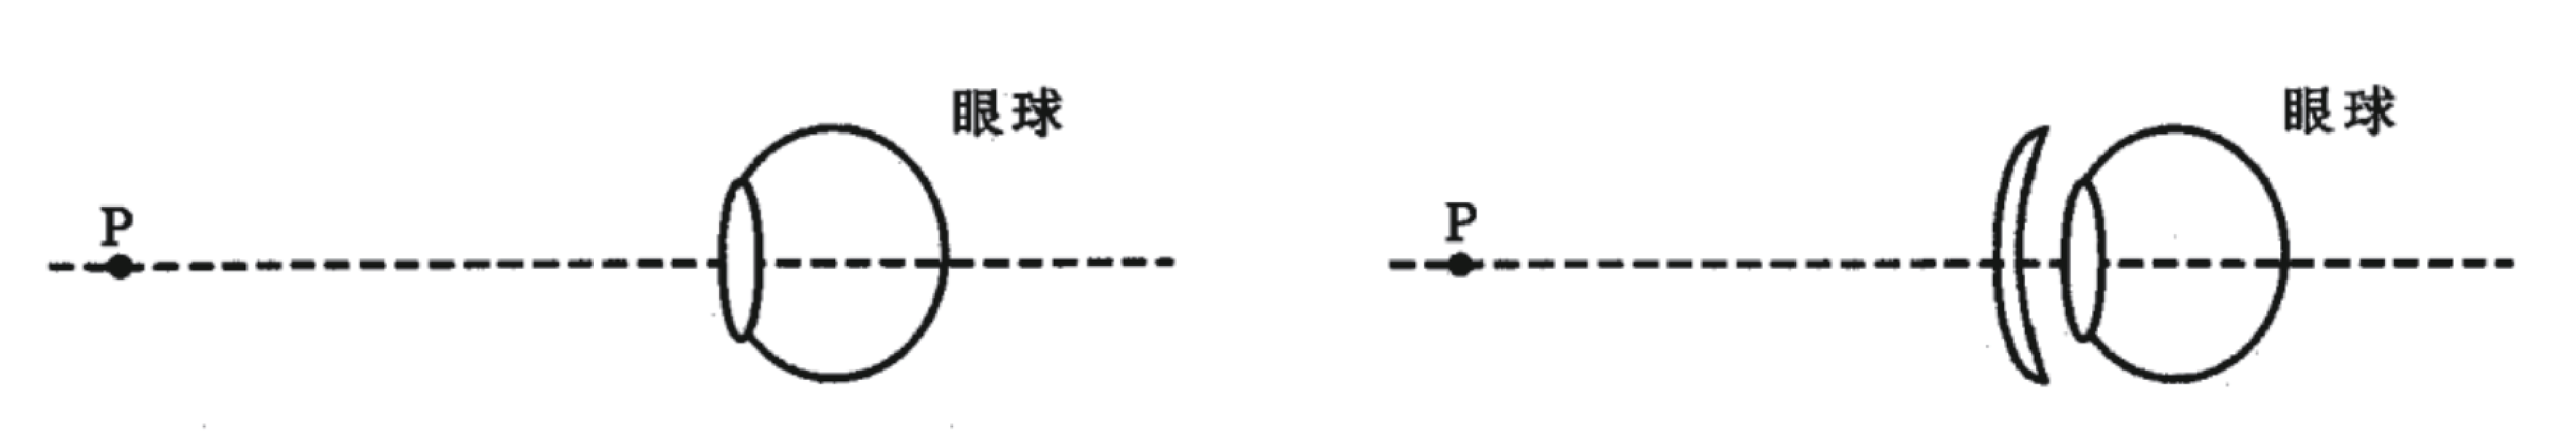
\includegraphics[width=0.95\textwidth]{images/opt-16.pdf}
	\end{center}
	\tagged{student}{\vspace*{4cm}}
	\begin{taggedblock}{teacher}
		\noindent
		解析:(1)(2)略。(3)33.3cm
	\end{taggedblock}
\end{example}
%%%%%%%%%%%%%%%%%%%%


从上面的例子可以看出,放大镜的放大倍数是很有限的,为了能够看到更小的物体就需要改进光学系统的设计。
为此目的人们发明了{\heiti 显微镜}(microscope),最简单的显微镜是由两个凸透镜构成,其光路如图所示。
靠近被观察物体的透镜称为{\heiti 物镜}(objective lens),它负责放大物体;根据透镜成像的规律可知,将物体放置于其一倍与二倍焦距之间将成一个放大,倒立的实像,但是一般来说这个实像与人眼的距离过近,小于明视距离使得我们无法观测。
为了看到这个放大的实像,需要利用另外一个透镜,它称为{\heiti 目镜}(eyepiece)。
将放大的实像放在目镜的一倍焦距以内,这样将成一个正立放大、位置合适的虚像以便肉眼来观测。

\begin{example}
已知简单显微镜物镜焦距为$f_1$,目镜焦距为$f_2$,证明显微镜的视角放大率
\[\beta = \frac{ L_0\Delta}{f_1f_2}\]
其中$\Delta = L-f_1-f_2$,$L$为显微镜镜筒的长度。
\tagged{student}{\vspace*{3cm}}
\begin{taggedblock}{teacher}
\newline
解析:实际使用当中,被测物体到显微镜的距离可调,但镜筒长度却不能够改变,设目镜成像过程当中物距为$u_1$,像距为$v_1$,根据成像公式可知对于给定的像距,物距和长度为$h$的物体的像的大小$h'$分别为
\[u_1=\frac{fv_1}{v_1-f} , \qquad h'=\frac{v_1}{u_1}h = \frac{v_1-f_1}{f_1}h \]
放大倒立的实像通过焦距为$f_2$的目镜观测的视角和放大镜一样,都是像高比上焦距,这样通过显微镜观测的视角为
\[
\theta = \frac{h'}{f_2} = \frac{v_1-f_1}{f_1f_2}h
\]
这样与同样的物体放在明视距离上观测的视角的比就是显微镜的视角放大率
\[
\beta = \frac{\theta}{h/L_0}=\frac{\frac{v_1-f_1}{f_1f_2}h}{h/L_0}=\frac{(v_1-f_1)L_0}{f_1f_2}= \frac{ L_0\Delta}{f_1f_2}
\]
其中最后一个等式来自于显微镜的结构。
从中可见镜筒越长、目镜物镜焦距越短显微镜的放大倍数就越大。
\end{taggedblock}
\end{example}


%%%%%%%%%%%%%
\begin{example}
	显微镜物镜组中常配有如图所示的透镜,它的表面是球面,左表面$S_1$的球心为$C_1$,半径为$R_1$,右表面$S_2$球心为$C_2$,半径为$R_2$,透镜玻璃对空气的折射率为$n$,两球心间的距离$C_1C_2=R_2/n$。
	在使用时,被观察的物位于$C_1$处,试证明
	
	1. 从物射向此透镜的光线经透镜折射后所有出射光线均相交于一点$Q$。
	
	2. $QC_2 = nR_2$
	
		\begin{flushright}
			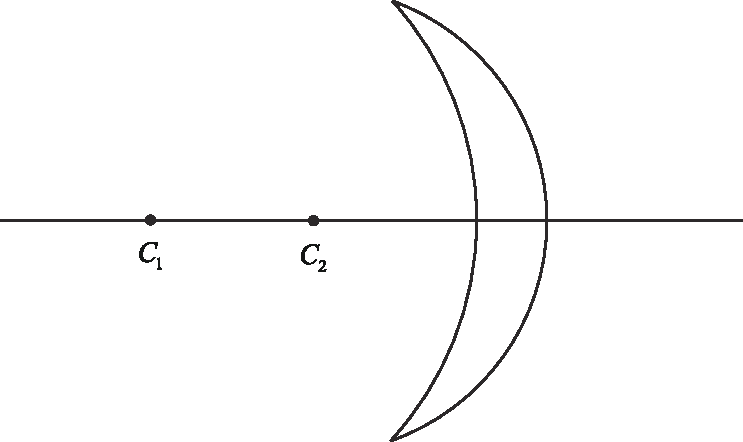
\includegraphics[width = 0.3\textwidth]{images/opt-12.pdf} 
		\end{flushright}
	\tagged{student}{\vspace*{4cm}}
	\begin{taggedblock}{teacher}
		\noindent
		解析:略
	\end{taggedblock}
\end{example}
%%%%%%%%%%%%%%%%%%%%


显微镜能够帮助我们看到那些很小的物体,与之相对应{\heiti 望远镜}(telescope)则是帮助人们看到那些遥远距离的物体。
我们知道当光源距离较远时它发出的光线可以近似认为是平行光,所有望远镜的设计思路都是使平行的入射光线通过反射或折射后再次变成平等的出射光线。
有限大小的物体发出的光会对人眼有一个微小的夹角,它发出的光通过望远镜之后如果张角变大,我们就有机会看到远处物体的细节。
依据物镜的性质望远镜又分为折射或反射式望远镜,其典型光路如图所示。

\begin{example}
简单望远镜由单个物镜和目镜构成,设其焦距分别为$f_1$和$f_2$。
试证明对于图所示的四类典型望远镜来说其放大率均为$\beta=f_1/f_2$,也就是说物镜焦距越长、目镜焦距越短的望远镜放大倍数越高。
\tagged{student}{\vspace*{4cm}}
\begin{taggedblock}{teacher}
\newline
解析:在放远镜的问题当中有一些近似,由于一般情况下物体距离观测者较远,所以有目镜成像时的物距$u_1\ll f_1$,这时肉眼看该物体的视角$\theta_0\simeq h/u_1$,无论是折射或反射式望远镜,其物镜成像的位置与物镜焦距的差别都十分之小,这样$v_1=\frac{f_1u_1}{u_1-f_1}\simeq f_1$。
像的大小则是
\[
h' = h\cdot \frac{v_1}{u_1}\simeq \frac{f_1}{u_1}
\]
所有种类的望远镜都是让物镜的像位于目镜的焦点位置,这样通过目镜观测该像的视角均为$\theta = \frac{h'}{f_2}$,联立以上各式可得放大率
\[
\beta=\frac{\theta}{\theta_0}=\frac{\frac{f_1}{uf_2}h}{\frac{h}{u_1}}=\frac{f_1}{f_2}
\]
\end{taggedblock}
\end{example}


%%%%%%%%%%%%%
\begin{example}
有两个凸透镜,它们的焦距分别为$ f_1$和$ f_2$,还有两个凹透镜,它们的焦距分别为$ f_3$	和$ f_4$,已知,$f_1>f_2>|f_3|>|f_4|$,如果要从这四个透镜中选取两个透镜,组成一架最简单的单筒望 远镜,要求能看到放大倍数尽可能大的正立的像,则应选焦距为\kong 的透镜作为物镜, 应选焦距为\kong 的透镜作为目镜。
	\tagged{student}{\vspace*{4cm}}
	\begin{taggedblock}{teacher}
		\newline
		解析:$f_1,f_4$
	\end{taggedblock}
\end{example}
%%%%%%%%%%%%%%%%%%%%





\begin{example}
太阳光被球形水滴经过如图所示的光路折射、反射、再折射以后射出形成彩虹。
将第一次折射的入射角记为$\alpha$,光线整体的偏转角记做$D$,很明显$D$依赖于$\alpha$的大小。
试给出它们的依赖关系并解释为什么太阳与彩虹的连线与人眼与彩虹的连线之间夹角约为$42^\circ$?
假设水对红光的折射率$n\simeq 4/3$,对其它颜色光的折射率稍大于红光。

\includegraphics[width=0.9\textwidth]{images/rainbow.pdf}
\tagged{student}{\vspace*{4cm}}
\begin{taggedblock}{teacher}
\newline
解析:根据折射定律,第一次折射的折射角$\beta$满足
\[
\beta = \arcsin\left (\frac{1}{n}\sin\alpha\right )
\]
连接BS,在三角形ABS当中根据几何条件可得偏转角与入射角的关系
\[
\alpha-\beta+\frac{D}{2}=\beta
\]
能够解得
\[ D(\alpha)=4\beta-2\alpha = 4\arcsin\left (\frac{1}{n}\sin\alpha\right )-2\alpha \]
不同的入射角$\alpha$对应于不同的偏转角,而那些最明亮的,能够最终被眼睛看到的光线集中在偏转方向最为集中的那些光线。
这种光线的条件是偏转角取极值,也就是$D$对$\alpha$的导数为零。
将它求导,可得
\[
\frac{dD(\alpha)}{d\alpha}=4\frac{\frac{1}{n}\cos\alpha}{\sqrt{1-(\frac{1}{n}\sin\alpha)^2}}-2=0
\]
将它整理整理化简可得
\[
\sin\alpha = \sqrt{\frac{4-n^2}{3}}\simeq\sqrt{\frac{20}{27}},\qquad \alpha\simeq 59.39^\circ,\qquad \beta\simeq 40.2^\circ
\]
在它基础上可以进一步算出偏转角
\[D =4\beta-2\alpha \simeq 42.02^\circ \]
也就是说对于红光来说当太阳与水滴的连线与视线成大约$42^\circ$时我们能够看到明亮的红光,对于其它的光线,它们的折射率与红光差别并不太大,也都集中在这个角度附近。
雨后当空气当中充满水滴以后我们就看到了彩虹。

\end{taggedblock}
\end{example}




